\documentclass{vkr}
\usepackage[english, russian]{babel} % переносы
\usepackage{graphicx} % для вставки картинок
\graphicspath{{images/}} % путь к изображениям
\usepackage[hidelinks]{hyperref}
\usepackage{float} % определяет метод H для рисунка с переносом на следующую страницу, ели не помещается
\usepackage{pdflscape}
\addto{\captionsrussian}{\renewcommand{\refname}{СПИСОК ИСПОЛЬЗОВАННЫХ ИСТОЧНИКОВ}}
\usepackage{xltabular} % для вставки таблиц
\usepackage{makecell}
\renewcommand\theadfont{} % шрифт в /thead
\usepackage{array} % для определения новых типов столбцов таблиц
\newcolumntype{T}{>{\centering\arraybackslash}X} % новый тип столбца T - автоматическая ширина столбца с выравниванием по центру
\newcolumntype{R}{>{\raggedleft\arraybackslash}X} % новый тип столбца R - автоматическая ширина столбца с выравниванием по правому краю
\newcolumntype{C}[1]{>{\centering\let\newline\\\arraybackslash\hspace{0pt}}m{#1}} % новый тип столбца C - фиксированная ширина столбца с выравниванием по центру
\newcolumntype{r}[1]{>{\raggedleft\arraybackslash}p{#1}} % новый тип столбца r - фиксированная ширина столбца с выравниванием по правому краю
\newcommand{\centrow}{\centering\arraybackslash} % командой \centrow можно центрировать одну ячейку (заголовок) в столбце типа X или p, оставив в оcтальных ячейках другой тип выравнивания
\newcommand{\finishhead}{\endhead\hline\endlastfoot}
\newcommand{\continuecaption}[1]{\caption*{#1}\\ \hline }
\usepackage{etoolbox}
\AtBeginEnvironment{xltabular}{\refstepcounter{tablecnt}} % подсчет таблиц xltabular, обычные таблицы подсчитываются в классе

\usepackage[tableposition=top]{caption} % подпись таблицы вверху
\captionsetup{strut=off}
\setlength{\intextsep}{0pt} % Vertical space above & below [h] floats
\setlength{\textfloatsep}{0pt} % Vertical space below (above) [t] ([b]) floats
\DeclareCaptionLabelFormat{gostfigure}{Рисунок #2} %подпись рисунка
\DeclareCaptionLabelFormat{gosttable}{Таблица #2} %подпись таблицы
\DeclareCaptionLabelSeparator{gost}{~--~} %разделитель в рисунках и таблицах
\captionsetup{labelsep=gost}
\captionsetup[figure]{aboveskip=10pt,belowskip=4mm,justification=centering,labelformat=gostfigure} % настройка подписи рисунка
\captionsetup[table]{font={stretch=1.41},skip=0pt,belowskip=0pt,aboveskip=8.5pt,singlelinecheck=off,labelformat=gosttable} % настройка подписи таблицы

\setlength{\LTpre}{8mm} % отступ сверху таблицы
\setlength{\LTpost}{6mm} % отступ снизу таблицы

\usepackage{enumitem}
\setlist{nolistsep,wide=\parindent,itemindent=*} % отступы вокруг списков, выравнивание с учетом разделителя

\usepackage{color} %% это для отображения цвета в коде
\usepackage{listings} %% листинги кода
\setmonofont[Scale=0.7]{Verdana} % моноширный шрифт для листинга

\definecolor{codegreen}{rgb}{0,0.6,0}
\definecolor{codegray}{rgb}{0.5,0.5,0.5}
\definecolor{codepurple}{rgb}{0.58,0,0.82}

\lstset{ %
language=C,                 % выбор языка для подсветки (здесь это С)
numbers=left,               % где поставить нумерацию строк (слева\справа)
numberstyle=\tiny,           % размер шрифта для номеров строк
stepnumber=1,                   % размер шага между двумя номерами строк
numbersep=5pt,                % как далеко отстоят номера строк от подсвечиваемого кода
commentstyle=\color{codegreen},
keywordstyle=\color{magenta},
numberstyle=\tiny\color{codegray},
stringstyle=\color{codepurple},
basicstyle=\linespread{0.95}\ttfamily,
backgroundcolor=\color{white}, % цвет фона подсветки - используем \usepackage{color}
showspaces=false,            % показывать или нет пробелы специальными отступами
showstringspaces=false,      % показывать или нет пробелы в строках
showtabs=false,             % показывать или нет табуляцию в строках
frame=single,              % рисовать рамку вокруг кода
tabsize=2,                 % размер табуляции по умолчанию равен 2 пробелам
captionpos=t,              % позиция заголовка вверху [t] или внизу [b] 
breaklines=true,           % автоматически переносить строки (да\нет)
breakatwhitespace=false, % переносить строки только если есть пробел
escapeinside={\%*}{*)}   % если нужно добавить комментарии в коде
}

\makeatletter % чтобы допускались русские комментарии в листингах
\lst@InputCatcodes
\def\lst@DefEC{%
 \lst@CCECUse \lst@ProcessLetter
  ^^80^^81^^82^^83^^84^^85^^86^^87^^88^^89^^8a^^8b^^8c^^8d^^8e^^8f%
  ^^90^^91^^92^^93^^94^^95^^96^^97^^98^^99^^9a^^9b^^9c^^9d^^9e^^9f%
  ^^a0^^a1^^a2^^a3^^a4^^a5^^a6^^a7^^a8^^a9^^aa^^ab^^ac^^ad^^ae^^af%
  ^^b0^^b1^^b2^^b3^^b4^^b5^^b6^^b7^^b8^^b9^^ba^^bb^^bc^^bd^^be^^bf%
  ^^c0^^c1^^c2^^c3^^c4^^c5^^c6^^c7^^c8^^c9^^ca^^cb^^cc^^cd^^ce^^cf%
  ^^d0^^d1^^d2^^d3^^d4^^d5^^d6^^d7^^d8^^d9^^da^^db^^dc^^dd^^de^^df%
  ^^e0^^e1^^e2^^e3^^e4^^e5^^e6^^e7^^e8^^e9^^ea^^eb^^ec^^ed^^ee^^ef%
  ^^f0^^f1^^f2^^f3^^f4^^f5^^f6^^f7^^f8^^f9^^fa^^fb^^fc^^fd^^fe^^ff%
  ^^^^20ac^^^^0153^^^^0152%
  % Basic Cyrillic alphabet coverage
  ^^^^0410^^^^0411^^^^0412^^^^0413^^^^0414^^^^0415^^^^0416^^^^0417%
  ^^^^0418^^^^0419^^^^041a^^^^041b^^^^041c^^^^041d^^^^041e^^^^041f%
  ^^^^0420^^^^0421^^^^0422^^^^0423^^^^0424^^^^0425^^^^0426^^^^0427%
  ^^^^0428^^^^0429^^^^042a^^^^042b^^^^042c^^^^042d^^^^042e^^^^042f%
  ^^^^0430^^^^0431^^^^0432^^^^0433^^^^0434^^^^0435^^^^0436^^^^0437%
  ^^^^0438^^^^0439^^^^043a^^^^043b^^^^043c^^^^043d^^^^043e^^^^043f%
  ^^^^0440^^^^0441^^^^0442^^^^0443^^^^0444^^^^0445^^^^0446^^^^0447%
  ^^^^0448^^^^0449^^^^044a^^^^044b^^^^044c^^^^044d^^^^044e^^^^044f%
  ^^^^0401^^^^0451%
  %%%
  ^^00}
\lst@RestoreCatcodes
\makeatother


% Режим шаблона (должен быть включен один из трех)
\ВКРtrue
%\Практикаtrue
%\Курсоваяtrue

\newcommand{\Дисциплина}{<<Проектирование и архитектура программных систем>>} % для курсовой
\newcommand{\КодСпециальности}{09.03.04} % Курсовая
\newcommand{\Специальность}{Программная инженерия} % Курсовая
\newcommand{\Тема}{Интерпретатор функционального языка программирования} % ВКР Курсовая
\newcommand{\ТемаВтораяСтрока}{с поддержкой метапрограммирования}
\newcommand{\ГдеПроводитсяПрактика}{Юго-Западном государственном университете} % для практики
\newcommand{\РуководительПрактПредпр}{} % для практики
\newcommand{\ДолжнРуководительПрактПредпр}{} % для практики
\newcommand{\РуководительПрактУнивер}{Чаплыгин А. А.} % для практики
\newcommand{\ДолжнРуководительПрактУнивер}{к.т.н. доцент} % для практики
\newcommand{\Автор}{Д. А. Антипов}
\newcommand{\АвторРод}{Антипова Д. А.}
\newcommand{\АвторПолностьюРод}{Антипова Дмитрия Александровича} % для практики
\newcommand{\Шифр}{20-06-0118}
\newcommand{\Курс}{4 } % для практики
\newcommand{\Группа}{ПО-02б}
\newcommand{\Руководитель}{А. А. Чаплыгин} % для ВКР и курсовой
\newcommand{\Нормоконтроль}{А. А. Чаплыгин} % для ВКР
\newcommand{\ЗавКаф}{А. В. Малышев} % для ВКР
\newcommand{\ДатаПриказа}{«04» апреля 2024~г.} % для ВКР
\newcommand{\НомерПриказа}{1616-с} % для ВКР
\newcommand{\СрокПредоставления}{«11» июня 2024~г.} % для ВКР, курсового

\begin{document}
\maketitle
\ifПрактика{}\else{
   \newpage
\begin{center}
\large\textbf{Минобрнауки России}

\large\textbf{Юго-Западный государственный университет}
\vskip 1em
\normalsize{Кафедра программной инженерии}
\vskip 1em
\ifВКР{
        \begin{flushright}
        \begin{tabular}{p{.4\textwidth}}
        \centrow УТВЕРЖДАЮ: \\
        \centrow Заведующий кафедрой \\
        \hrulefill \\
        \setarstrut{\footnotesize}
        \centrow\footnotesize{(подпись, инициалы, фамилия)}\\
        \restorearstrut
        «\underline{\hspace{1cm}}»
        \underline{\hspace{3cm}}
        20\underline{\hspace{1cm}} г.\\
        \end{tabular}
        \end{flushright}
        }\fi
\end{center}
\vspace{1em}
  \begin{center}
  \large
\ifВКР{
ЗАДАНИЕ НА ВЫПУСКНУЮ КВАЛИФИКАЦИОННУЮ РАБОТУ
  ПО ПРОГРАММЕ БАКАЛАВРИАТА}
  \else
ЗАДАНИЕ НА КУРСОВУЮ РАБОТУ (ПРОЕКТ)
\fi
\normalsize
  \end{center}
\vspace{1em}
{\parindent0pt
  Студента \АвторРод, шифр\ \Шифр, группа \Группа
  
1. Тема «\Тема\ \ТемаВтораяСтрока»
\ifВКР{
утверждена приказом ректора ЮЗГУ от \ДатаПриказа\ № \НомерПриказа
}\fi.

2. Срок предоставления работы к защите \СрокПредоставления

3. Исходные данные для создания программной системы:

3.1. Перечень решаемых задач:}

\renewcommand\labelenumi{\theenumi)}

\begin{itemize}
	\item провести анализ предметной области;
	\item спроектировать функциональный язык программирования с поддержкой метапрограммирования;
	\item спроектировать интерпретатор этого языка;
	\item выбрать технологии и методики для реализации интерпретатора;
	\item реализовать интерпретатор средствами языка программирования \quotes{C} и ОС \quotes{GNU/Linux}.
\end{itemize}

{\parindent0pt
  3.2. Входные данные и требуемые результаты для программы:}

\begin{enumerate}
\item Входными данными для программной системы является файл с кодировкой \quotes{UTF-8}, содержащий программный код на разработанном в рамках этой работы языке программирования.
\item Выходными данными для программной системы является результат выполнения переданного в программную систему программного кода.
\end{enumerate}

{\parindent0pt

  4. Содержание работы (по разделам):
  
  4.1. Введение
  
  4.1. Анализ предметной области
  
4.2. Техническое задание: основание для разработки, назначение разработки,
требования к программной системе, требования к оформлению документации.

4.3. Технический проект: общие сведения о программной системе, обоснование выбора технологии, проектирование архитектуры программной системы.

4.4. Рабочий проект: перечень разработанных модулей, спецификация компонентов и модулей программной системы, тестирование программной системы, сборка компонентов программной системы.

4.5. Заключение

4.6. Список использованных источников

5. Перечень графического материала:

\списокПлакатов

\vskip 2em
\begin{tabular}{p{6.8cm}C{3.8cm}C{4.8cm}}
Руководитель \ifВКР{ВКР}\else работы (проекта) \fi & \lhrulefill{\fill} & \fillcenter\Руководитель\\
\setarstrut{\footnotesize}
& \footnotesize{(подпись, дата)} & \footnotesize{(инициалы, фамилия)}\\
\restorearstrut
Задание принял к исполнению & \lhrulefill{\fill} & \fillcenter\Автор\\
\setarstrut{\footnotesize}
& \footnotesize{(подпись, дата)} & \footnotesize{(инициалы, фамилия)}\\
\restorearstrut
\end{tabular}
}

\renewcommand\labelenumi{\theenumi.}

   \abstract{РЕФЕРАТ}

Объем работы равен \formbytotal{lastpage}{страниц}{е}{ам}{ам}. Работа содержит \formbytotal{figurecnt}{иллюстраци}{ю}{и}{й}, \formbytotal{tablecnt}{таблиц}{у}{ы}{}, \arabic{bibcount} библиографических источников и \formbytotal{числоПлакатов}{лист}{}{а}{ов} графического материала. Количество приложений – 2. Графический материал представлен в приложении А. Фрагменты исходного кода представлены в приложении Б.

Перечень ключевых слов: коммерческий сайт, Система, CMS, Битрикс, Joomla, аддитивные технологии, 3D-принтеры, услуги, сервисы, информатизация, автоматизация, информационные технологии, веб-форма,  Apache, классы, база данных, средства защиты информации, подсистема, компонент, модуль, сущность, информационный блок, метод, контент-редактор, администратор, пользователь, web-сайт.

Объектом разработки является web-сайт компании,  занимающейся производством 3D-принтеров, выпуском оборудования для создания порошков, разработкой программного обеспечения и организацией центров аддитивного производства.

Целью выпускной квалификационной работы является привлечение клиентов, увеличение заказов, информирование о продукции и услугах путем создания сайта компании.

В процессе создания сайта были выделены основные сущности путем создания информационных блоков, использованы классы и методы модулей, обеспечивающие работу с сущностями предметной области, а также корректную работу web-сайта, разработаны разделы, содержащие информацию о компании, ее деятельности, производимой продукции и услугах, разработан сервис по заказу 3D-деталей.

При разработке сайта использовалась система управления контентом "<1С-Битрикс: Управление сайтом">.

Разработанный сайт был успешно внедрен в компании.

\selectlanguage{english}
\abstract{ABSTRACT}
  
The volume of work is \formbytotal{lastpage}{page}{}{s}{s}. The work contains \formbytotal{figurecnt}{illustration}{}{s}{s}, \formbytotal{tablecnt}{table}{}{s}{s}, \arabic{bibcount} bibliographic sources and \formbytotal{числоПлакатов}{sheet}{}{s}{s} of graphic material. The number of applications is 2. The graphic material is presented in annex A. The layout of the site, including the connection of components, is presented in annex B.

List of keywords: commercial website, System, CMS, Bitrix, Joomla, additive technologies, 3D printers, services, services, informatization, automation, information technology, web form, Apache, classes, database, component, module, entity, information block, method, content editor, administrator, user, web site.

The object of the research is the analysis of information technologies for the development of a production company's website.

The object of the development is the website of a company engaged in the production of 3D printers, the production of equipment for the creation of powders, software development and the organization of additive manufacturing centers.

The purpose of the final qualifying work is to attract customers, increase orders, inform about products and services by creating a company website.

In the process of creating the site, the main entities were identified by creating information blocks, classes and methods of modules were used to ensure work with the entities of the subject area, as well as the correct operation of the website, sections containing information about the company, its activities, products and services were developed, a service for ordering 3D parts was developed.

When developing the site, the content management system <<1C – Bitrix: Site Management>> was used.

The developed website was successfully implemented in the company.
\selectlanguage{russian}
}\fi
\tableofcontents
\section*{ОБОЗНАЧЕНИЯ И СОКРАЩЕНИЯ}

ИТ -- информационные технологии.

ПО -- программное обеспечение.

ПС -- программная система.

ЯП -- язык программирования.

ДЯП -- демонстрационный язык программирования.

ЛА -- лексический анализатор.

СА -- синтаксический анализатор.

UML (Unified Modelling Language) -- язык графического описания для объектного моделирования в области разработки программного обеспечения.
\ifПрактика{}\else{\section*{ВВЕДЕНИЕ}
\addcontentsline{toc}{section}{ВВЕДЕНИЕ}

Парадигма метапрограммирования уже многие годы активно используется при разработке гибкого и адаптивного программного обеспечения, обеспечивая одни программы возможностью генерировать и трансформировать другие или самих себя, тем самым позволяя сокращать исходный код и одновременно с тем повышая его конфигурируемость и масштабируемость.

Со временем сложность программ возрастает, их функциональные возможности становятся более обширными, а требования к мобильности растут. Метапрограммирование может выступать как эффективный инструмент по снижению влияния таких требований на скорость и сложность разработки. В результате программисты могут писать ПО, формирующее программный код с учётом внешних условий и на основе предъявляемых требований.

Ещё одним популярным подходом, эффективным для решения всё тех же проблем и хорошо сочетаемым с генерацией кода, выступает функциональная парадигма программирования. Языки, берущие её за основу, приобрели значительную востребованность в последние годы благодаря своей способности обеспечивать более предсказуемый и прозрачный, легко анализируемый, модульный код. Поддержка функций высшего порядка и следование принципу неизменяемости данных также выделяют их как разумный вариант для разработок с такими требованиями.

Включая метапрограммирование в функциональный язык, производится заметное повышение потенциала языка к достижению поставленных разработкой целей \cite{e31}. Удачность симбиоза этих идей, наряду с другими успешными решениями, привела к тому, что языки, такие как Haskell, F\#, Erlang, OCaml, Lisp и Clojure стали превосходящими в индустрии, где требования к надежности и адаптивности систем высоки, а многие языки, изначально не имевшие таких возможностей, получают их частичную или полную поддержку \cite{e30}.

В этой выпускной квалификационной работе будет спроектирован функциональный язык программирования с поддержкой метапрограммирования и программная система для выполнения кода на этом языке - транслятор типа интерпретатор. Интерпретатор читает исходный код программы, анализирует и исполняет его инструкции, выводя результаты на экран или в файл. В отличие от компилятора \cite{e3}, который переводит весь код программы в машинный, интерпретатор обрабатывает его по одной инструкции, тем самым выполняя программы без предварительной компиляции. Язык, разработанный для этого интерпретатора, ставит минимализм и выразительность синтаксиса в приоритет, гарантируя, что основные концепции функционального программирования и метапрограммирования доступны и удобны в использовании.

Цель настоящей работы – разработка программной системы, позволяющей сокращение размера исходного кода программ за счёт метапрограммирования. Для достижения поставленной цели необходимо решить следующие задачи:
\begin{itemize}
	\item провести анализ предметной области;
	\item спроектировать функциональный язык программирования с поддержкой метапрограммирования;
	\item спроектировать интерпретатор этого языка;
	\item выбрать технологии и методики для реализации интерпретатора;
	\item реализовать интерпретатор средствами языка программирования \quotes{C} и ОС \quotes{GNU/Linux}.
\end{itemize}

\emph{Структура и объем работы.} Отчет состоит из введения, 4 разделов основной части, заключения, списка использованных источников, 2 приложений. Текст выпускной квалификационной работы равен \formbytotal{page}{страниц}{е}{ам}{ам}.

\emph{Во введении} сформулирована цель работы, поставлены задачи разработки, описана структура работы, приведено краткое содержание каждого из разделов.

\emph{В первом разделе} на стадии описания технической характеристики предметной области приводится сбор информации о технологиях и методиках, необходимых для реализации программной системы.

\emph{Во втором разделе} на стадии технического задания приводятся требования к разрабатываемому интерпретатору и языку.

\emph{В третьем разделе} на стадии технического проектирования представлены проектные решения для интерпретатора.

\emph{В четвертом разделе} приводится список модулей и их полей и методов, созданных при разработке, а также производится тестирование разработанного интерпретатора.

В заключении излагаются основные результаты работы, полученные в ходе разработки.

В приложении А представлен графический материал.
В приложении Б представлены фрагменты исходного кода. 
}\fi
\section{Анализ предметной области}

\subsection{Понятие интерпретатора}

Интерпретатор языка программирования -- это программа типа транслятор, считывающая программный код, написанный на определённом языке программирования, по одной инструкции или группе инструкций и немедленно исполняющая их в соответствии с синтаксисом и семантикой языка.

В сравнении с компилятором, анализирующим и единоразово преобразующим весь исходный код программы в машинный код перед её выполнением, и JIT-компилятором, выполняющим компиляцию во время исполнения, интерпретатор в реальном времени анализирует и выполняет код по одной инструкции, сначала преобразуя её во внутреннее представление и затем в машинный код.



\subsection{Строение интерпретатора}

\subsubsection{Лексический анализатор и лексема}
Всё начинается с лексемы — символа или набора символов, минимально значимой единицы исходного кода, которую интерпретатор может распознать и обработать. Лексемы включают в себя ключевые слова, идентификаторы, константы, символы и операторы. Они служат для разделения кода на части, которые затем будут преобразованы во внутреннее представление интерпретатора и выполнены им.

С применением лексического анализатора лексемы постепенно перерабатываются в токены.

Токен -- та же лексема, но представленная специальным значением или имеющая дополнительный атрибут, что позволит синтаксическому анализатору идентифицировать её или узнать о ней дополнительную информацию. Например, тип лексемы -- число, строка и так далее.

Лексический анализ (токенизация) -- формирование токенов на основе исходного кода программы, таких как ключевые слова, идентификаторы, операторы, литералы и так далее. 

Лексический анализатор (ЛА) распознаёт лексемы в исходном коде программы, пропуская пустоты (пробелы, переводы строк), определяет особенности лексемы и из полученных данных формирует токен, который будет передан следующим компонентам интерпретатора. Считывание текста программы из потока ввода производится до тех пор, пока не встретится зарезервированный символ, после чего начинается формирование токена. Либо, если в синтаксисе языка предусмотрены односимвольные лексемы, то формирование происходит сразу. Также лексический анализатор берёт на себя задачу по выявлению символов, не являющихся частью синтаксиса языка в анализируемом контексте, и при обнаружении таковых выводит на экран соответствующую ошибку.



\subsubsection{Синтаксический анализатор, синтаксис языка программирования и внутреннее представление}

Следующим этапом работы интерпретатора является анализ полученных от лексического анализатора токенов и преобразование их во внутреннее представление интерпретатора для передачи следующим его компонентам.

Внутреннее представление -- это проекция выражений и конструкций языка программирования внутри интерпретатора. Им определяется как интерпретатор хранит данные и оперирует ими во время выполнения программы.

Синтаксис языка программирования представляет собой набор правил для написания языковых выражений и конструкций, которые будут интерпретированы и выполнены компилятором или интерпретатором соответствующего языка ровно таким образом, каким это описано в спецификации языка.

Синтаксис определяет как символы образуют лексемы и как они комбинируются для формирования языковых конструкций и выражений, которые затем интерпретируются компьютером. Он определяет порядок операций, приоритет операторов, структуру программы, а также способы объявления переменных, функций, ветвлений и других конструкций, составляющих структуру программного кода. При отсутствии ошибок в реализации интерпретатора, несоблюдение или неполное понимание синтаксических правил может привести как к ошибкам, так и к неожиданному с точки зрения разработчика поведению.

Синтаксический анализатор (СА) отвечает за анализ синтаксиса программного кода, проверку его на соответствие правилам и построение в соответствии с синтаксисом языка программирования объектов внутреннего представления интерпретатора на основе полученного от лексического анализатора токена.

Если обнаруживается ошибка в синтаксисе программы, то этот анализатор выводит на экран соответствующее сообщение об ошибке и прекращает дальнейшую обработку программы. Такой ошибкой может быть, например, отсутствующая закрывающая скобка или ключевое слово, которое отсутствует в языке программирования.



\subsubsection{Исполнитель}

После успешного завершения синтаксического анализа и получения сформированных СА объектов, они передаются на исполнение.

Исполнение -- выполнение кода, представленного во внутреннем формате, пошаговое выполнение инструкций программы, обрабатывая операторы и вычисляя значения выражений.

В процессе исполнения интерпретатор манипулирует теми объектами, которые ранее были сформированы синтаксическим анализатором из токенов. Именно на этапе исполнения происходят все вычисления и работа с данными программы -- объявление переменных и задание им значений, вызов функций и так далее.

Таким образом, исполнитель, выполняющий исполнение внутреннего представления, можно назвать ключевым компонентом интерпретатора.


\subsubsection{Сборщик мусора}
Сборщик мусора — это компонент интерпретатора, который отслеживает неиспользуемые объекты внутреннего представления и освобождает занятую ими память.

Неиспользуемыми объектами считаются те, которых нельзя достичь перемещаясь по дереву ссылок от активных объектов.

В зависимости от целей, поставленных разработчиком, наличие сборщика мусора может быть как положительной, так и отрицательной чертой языка программирования. Если вопрос занимаемой программой ОЗУ не является особенно важным, его наличие освобождает программиста от необходимости в ручном режиме выделять и освобождать память, что значительно упрощает процесс разработки, сводит к минимуму потенциальные уязвимости и проблематику утечек памяти в разрабатываемом ПО.


\subsection{Функциональное программирование}

Функциональное программирование -- это парадигма разработки ПО, где функции выступают в роли основного элемента конструкции программ и могут в качестве аргументов принимать другие функции. Тем самым выстраивается структура, основанная на функциях, их взаимодействии и композиции.

Также в этой парадигме принята идея о том, что по возможности и если то будет разумным, стоит придерживаться написания "чистых" функций -- функций, не имеющих побочных эффектов и при вызове с одними и теми же аргументами всегда возвращающих одинаковый результат, без изменения состояния программы или лексического окружения.

Но, для поддержания чистоты функций, стоит по возможности следовать концепции неизменности данных, суть которой заключается в отказе от изменения каких-либо уже сформированных данных. Таким образом, предпочтение отдаётся написанию функций, которые не изменяют исходные данные, а формируют и возвращают новые на основе исходных. Оба эти подхода способствуют формированию модульного, предсказуемого и надёжного кода, что в последствии упростит отладку и тестирование программы.

Основу для реализации функциональной парадигмы составляют функции высшего порядка и лямбда-функции.

Функции, имеющие возможность принимать в качестве аргументов другие функции, тем самым формируя цепи функциональных преобразований, где одни функции могут быть переданы и манипулируемы подобно другим объектам языка вроде списков или чисел, называются функциями высшего порядка. Умелое использование таких возможностей для создания обобщённых функций, применяемых для выполнения более широкого спектра условий, приводит к повышению модульности, переиспользуемости и выразительности кода.

Лямбда-функции (анонимные функции) -- это безымянные функции высшего порядка, которые используют в качестве аргумента для передачи другим функциям, возврата функции из функции или одноразового применения, что позволяет без необходимости не занимать пространство имён.

\subsection{Метапрограммирование}
Метапрограммирование — это вид программирования, который связан с созданием программ, генерирующих другие программы как результат своей работы, или программ, изменяющих себя во время выполнения. В функциональном программировании такой подход используется часто, потому как функции сами являются данными и могут быть переданы как аргументы другим функциям, создавать новые функции и изменять собственные тела.

Метапрограммирование реализуется системой макросов, позволяющей разработчику создавать новые языковые конструкции, генерируя, изменяя и делая динамическим код программы.

Макросы -- это функции, генерирующие код, который в последствии заменит код генерации. Они работают на этапе компиляции или интерпретации, позволяя трансформировать исходный код перед его выполнением. Макросы позволяют создавать собственные синтаксические конструкции и расширять язык, что открывает для разработчика почти безграничные возможности по адаптации языка под свои нужды и создания адаптивного ПО. 

Например, макросы можно применить для включения или исключения частей кода в зависимости от условий запуска и особенностей компьютера, на котором происходит запуск. Помимо прочего, использование макросов может ускорить работу программ за счёт возможности один раз сгенерировать функцию с определёнными аргументами, а после переиспользовать её, без необходимости каждый раз заново вызывать функцию с одними и теми же аргументами.

\subsection{Язык программирования Lisp}

Функциональный язык программирования с уклоном в сферу разработки искусственного интеллекта, один из самых старых используемых и теперь языков — Lisp, появившийся в 1958 трудами учёного Джона Маккарти.

Инновационность языка состояла в том, что его автор спроектировал удобный инструментарий для работы со списками и символами, что было очень востребовано при решении задач обработки естественного языка и символьной логики. Список в Lisp -- главный элемент, потому как весь программный код на нём в конечном итоге состоит из множества списков. Хотя в первое время Lisp использовался только для решения неширокого перечня задач в сфере искуственного интеллекта, спустя чуть более чем десять лет с момента создания он всё же получил широкую известность и на долгое время стал центральным в этой сфере.

Кроме того, наличие успешной реализации системы макросов, составляющей в нём основу парадигмы метапрограммирования, в сумме с другими преимуществами сделала его востребованным для разработки предметно-ориентированных языков. Суть языков такого типа заключается в их адаптированности под конкретные задачи и способы применения, способствуя таким образом удобству написания программного кода.

Также примечательным является, что сборщик мусора и возможность использовать функции подобно данным впервые были введены именно в этом языке. 

Постепенно оригинальный Lisp отходил на второй план и известность перенимали его диалекты. На данный момент одним из наиболее используемых является Common Lisp — диалект, ставящий своей целью объединение удачных решений других разновидностей оригинального языка, чтобы сформировать мультипарадигменную, очень гибкую и достаточно широкую в плане способов применения и базовой функциональности вариацию.
\section{Техническое задание}
\subsection{Основание для разработки}

Полное наименование системы: \quotes{Интерпретатор функционального языка программирования с поддержкой метапрограммирования}.

Основанием для разработки программы является приказ ректора ЮЗГУ от «15» апреля 2024 г. №1779-с «Об утверждении тем выпускных квалификационных работ».

\subsection{Цель и назначение разработки}

Цель этой работы -- разработка программной системы, позволяющей сокращение размера исходного кода программ за счёт метапрограммирования.

Для достижения этой цели было принято решение разработать интерпретатор функционального языка программирования с поддержкой метапрограммирования. Основной задачей разработки является разработка программного обеспечения, способного анализировать и исполнять программы, написанные на функциональном языке программирования, а также обеспечивать возможности генерации и изменения кода на этом языке с использованием инструментов метапрограммирования.

Интерпретатор, созданный в рамках данной работы, должен иметь все ключевые функции, обеспечивающие поддержку парадигм метапрограммирования и функционального программирования. Для их реализации будет разработан простой и минималистичный функциональный язык программирования, называемый \quotes{демонстрационный язык программирования} (ДЯП), поддерживающий метапрограммирование.

Таким образом, интерпретатор сможет работать с  числами, строками, переменными, функциями, лямбда-выражениями, макросами и другими необходимыми конструкциями, обеспечивающими разработчику возможность использовать метапрограммирование для создания адаптивных и реплицируемых приложений.

Задачами данной разработки являются:
\begin{itemize}
	\item провести анализ предметной области;
	\item спроектировать функциональный язык программирования с поддержкой метапрограммирования, являющийся подмножеством языка \quotes{Common Lisp};
	\item спроектировать интерпретатор этого языка;
	\item выбрать технологии и методики для реализации интерпретатора;
	\item реализовать интерпретатор средствами языка программирования \quotes{C} и ОС \quotes{GNU/Linux}.
\end{itemize}


\subsection{Описание разрабатываемого языка}

Разрабатываемый язык является подмножеством языка программирования \quotes{Common Lisp} и сосредотачивается на реализации его базовых возможностей по работе с данными и метапрограммирования. Потому, он будет иметь функциональность для работы с переменными, функциями, лямбда-выражениями, функциями высшего порядка, числами, строками, символами, списками и массивами. Введутся базовые функции для обработки данных, включая операции сложения чисел, выделения подстрок из строк, определения имени символа по символьному объекту и другие, реализующие минимально необходимые возможности для манипуляции данными. Также будет включена система макросов как основной элемент реализации метапрограммирования.

\subsubsection{Алфавит языка}
Алфавит языка программирования -- это перечень символов, допустимых к использованию для записи синтаксических конструкций этого языка \cite{e4}. Символом может быть как буква, цифра или знак препинания, так и любой другой знак, рассматриваемый как неделимый элемент языка.

Алфавит разработанного языка включает:
\begin{itemize}
	\item латинские символы верхнего и нижнего регистра;
	\item римские цифры;
	\item символы, зарезервированные под описание конструкций языка, перечисленные через пробел: ' ` , . '' \#;
	\item другие символы, перечисленные через пробел: + - * / = \_ \& | < >.
\end{itemize}

\subsubsection{Лексемы, распознаваемые лексическим анализатором}

Список наименований лексем, распознаваемых лексическим анализатором, а также их символьное представление или пример:
\begin{itemize}
	\item десятичное и шестнадцатеричное целое число: 10, 0xFFAA;
	\item вещественное число: 1.34;
	\item символ: A;
	\item цитата: ';
	\item квазицитата: `;
	\item запятая: ,;
	\item запятая-at: ,@;
	\item решётка: \#;
	\item левая скобка: (;
	\item правая скобка: );
	\item точка: .;
	\item строка: \quotes{a b c v ddd};
	\item неизвестный объект -- объект, который ЛА не смог определить;
	\item конец потока.
\end{itemize}

Помимо этого, для удобства разработчика, синтаксисом языка предусмотрена возможность добавлять в код комментарии. Комментарий начинается со знака ‭\quotes{;} и заканчивается переносом строки.

Символ \quotes{\textbackslash} используется для экранирования.


\subsubsection{Типы данных}
Для языка программирования были определены шесть фактических типов данных и два псевдотипа:
\begin{itemize}
	\item число -- десятичные и шестнадцатеричные числа, размер которых ограничен 28 битами (от -134217728 до 134217727). Например: 10, 0xFFAA;
	
	\item большое число -- число, для хранения которого выделено 32 бит. Например: 134217728;
	
	\item строка -- произвольный набор алфавитных символов, задающийся в двойных кавычках. Например: \quotes{ab 12 /};
	
	\item символ -- именованный нечувствительно к регистру объект, который может указывать на некоторое значение -- число, лямбда-выражение, макрос, строку, массив, список или функцию. Имя символа должно начинаться с буквы или разрешенного символа и может содержать буквы, цифры, символы. Таким образом, переменные, функции и другие объекты языка, к которым можно обращаться по имени, являются символами, содержащими указатель на объект с данными, заданными для этого символа. Пример символа: 'A;
	
	\item точечная пара (список) -- это хранилище, содержащее только два элемента, называемые левым и правым. Пара носит название точечной, так как в синтаксисе эта конструкция представляет собой два элемента, разделённые точкой, обрамлённые в круглые скобки. Элементом пары может быть другая пара, что позволяет создавать списки, выстроенные из цепи точечных пар. Правый элемент последнего элемента такой цепи указывает на специальное значение nil. Например: ('a . (4 . nil));
	
	\item массив -- хранилище с прямым доступом к элементам (можно обращаться по индексу), содержащее ноль или более атомов, разделенных пустотами и заключённых в круглые скобки, перед открывающей ставится \#. Массивы могут содержать в себе другие массивы. Пример: \#(3 6 9).
\end{itemize}

Для идентификации типов в интерпретаторе будет использоваться перечисление, содержащее следующие значения:
\begin{itemize}
	\item NUMBER: число;
	\item BIGNUMBER: большое число;
	\item SYMBOL: символ;
	\item PAIR: точечная пара (список);
	\item STRING: строка;
	\item ARRAY: массив.
\end{itemize}

S-выражение -- это основной элемент синтаксиса языка, который может быть атомом или списком. S-выражения нечувствительны к регистру. Все инструкции в ДЯП являются s-выражениями, из чего следует, что программный код представляет собой множество s-выражений \cite{e10}.

Атом -- псевдотип, специальное название для обозначения примитивных объектов данных, которые не разбиваются на составляющие: символы, числа и строки.

Для обозначения \quotes{истинного} и \quotes{ложного} используются зарезервированные объекты-символы \quotes{T} и \quotes{NIL} соответственно.

\subsubsection{Функции и лямбда-выражения}

В языке программировании применяются функции и лямбда-выражения.

Функция представлена в виде списка, содержащего символ, имя которого соответствует имени функции, список аргументов и тело функции.

Для объявления новой функции используется функция defun, имеющая следующий синтаксис:

\quotes{(defun name (p \textsubscript 1 ... p \textsubscript n) e)}, где name -- имя объявляемой функции, p \textsubscript 1 ... p \textsubscript n -- параметры функции, e -- тело функции.

Вызов функции -- список, где первый элемент это имя функции, а последующие являются её аргументами.

Синтаксис вызова функции:

\quotes{(name a \textsubscript 1 ... a \textsubscript n)}, где name -- имя вызываемой функции, а a \textsubscript 1 ... a \textsubscript n -- передаваемые функции аргументы.

Лямбда-выражения объявляются идентично функциям, но вместо функции defun используется lambda и, так как лямбда-выражения безымянны, имя не задаётся.

Для вызова лямбда-выражения необходимо создать список, где первым элементом будет само лямбда-выражение, а a \textsubscript 1 ... a \textsubscript n -- передаваемые выражению аргументы: 

\quotes{((lambda (p \textsubscript 1 ... p \textsubscript n) e) a \textsubscript 1 ... a \textsubscript n)}.

При вызове, сначала вычисляются все аргументы a \textsubscript 1 ... a \textsubscript n. Затем каждому параметру p \textsubscript 1 ... p \textsubscript n ставится в соответствие вычисленное значение аргументов a \textsubscript 1 ... a \textsubscript n. После этого вычисляется выражение e, содержащее параметры, вместо которых будут подставлены их значения. Например:

\begin{lstlisting}[language=Lisp, frame=none]
< ((lambda (x y) (cons x (cdr y))) 'z '(a b c))
> (Z B C)
\end{lstlisting}

Это лямбда-выражение с помощью функции cons создаёт список, состоящий из значения аргумента x и обрезанного со второго элемента с помощью cdr списка y. Результатом выполнения этого кода будет новый список -- \quotes{(Z B C)}.

Также имеется возможность объявить параметр функции таким образом, чтобы он собирал все аргументы, начинающиеся с соответствующего ему, в список. Для этого перед таким параметром через пробел помещается конструкция \quotes{\&rest}. Например:

\begin{lstlisting}[language=Lisp, frame=none]
< (defun test (a b &rest c) (+ a (+ b (car c))))
< (test 1 2 3 4 5)
> 6
\end{lstlisting}

В результате в переменную \quotes{c} попадут числа 3, 4 и 5. Так как \quotes{a} равна 1, \quotes{b} равна 2, а \quotes{car c} вернёт \quotes{3} - вычисленное значение - 6. Такая возможность позволяет разрабатывать функции с динамическим числом переменных, что имеет большое значение в разработке адаптивного ПО.

Функции и лямбда-выражения могут быть получены и переданы в качестве аргументов или возвращены из функции и лямбда-выражения, как и необходимо в функциональной парадигме программирования. Иначе говоря, реализована поддержка функций высшего порядка.

\subsubsection{Макросы}

В ДЯП для создания макросов применяется функция defmacro, а также операторы quote, backquote и comma.

Функция defmacro имеет следующий синтаксис:
\quotes{(defmacro name (a \textsubscript 1 ... a \textsubscript n) e)}, где name -- имя макроса, a \textsubscript 1 ... a \textsubscript n -- параметры макроса, e -- тело макроса.

Пример использования:

\begin{enumerate}
	\item Создам макрос, задающий шаблон для генерации выражения:
	
	\begin{lstlisting}[language=Lisp, frame=none]
	(defmacro test (var val) (list 'defvar var val))}
	\end{lstlisting}
	
	При вычислении этот макрос заменится списком, первым элементом которого будет символ defvar для объявления переменной, а последующими -- переданные при вызове макроса аргументы:
	
	\begin{lstlisting}[language=Lisp, frame=none]
	(defvar var val)}
	\end{lstlisting}
	
	Для того, чтобы посмотреть что собой будет представлять вычисленный макрос с переданными ему аргументами, имеется функция \quotes{macroexpand}, куда вызов макроса передаётся в виде списка, на который применено цитирование:
	
	\begin{lstlisting}[language=Lisp, frame=none]
	< (macroexpand '(test a 2))
	> (defvar a 2)
	\end{lstlisting}
	
	\item Вызову макрос с символом \quotes{abc} и числом 100 в качестве аргумента. При вызове происходит вычисление тела макроса (развертывание макроса):
	
	\quotes{(test abc 100)} преобразуется в \quotes{(defvar abc 100)}.
	
	\item Получившееся выражение вычисляется. Список расценивается как код, который определяет переменную и присваивает ей значение:
	
	\begin{lstlisting}[language=Lisp, frame=none]
	(defvar abc 100)
	\end{lstlisting}
\end{enumerate}

По итогу был создан макрос test, объявляющий переменную с именем, переданным ему в качестве первого аргумента, и значением в качестве второго.

Кавычки (') -- символ, используемый для реализации цитирования -- предотвращения вычисления выражения. Например, выражение (* 2 2) будет автоматически вычислено и даст 4, в то время как '(* 2 2) будет восприниматься как список символов.

Но для предоставления по-настоящему широкого спектра возможностей для разработчика, необходимо реализовать инструментарий, позволяющий выполнять частичные вычисления -- квазицитирование.

Для того будут использоваться символы обратной кавычки \quotes{`} и запятой \quotes{,}. Обратная кавычка будет указывать на то, что выражение содержит вычисляемые элементы, а запятая укажет на них.

Пример использования:
\begin{lstlisting}[language=Lisp, frame=none]
< (defvar b 12) (print `(+ a ,b))

> (+ A 12)
\end{lstlisting}

Таким образом, \quotes{+} и \quotes{a} были восприняты интерпретатором как символы и остались невычисленными, а \quotes{b} заменён значением соответствующей переменной.

Также необходимой является функция развёртывания списков, обозначаемая лексемой \quotes{,@} (запятая-собачка). Если поместить её перед списком, после вычисления скобки, обрамляющие список, будут удалены и элементы списка предстанут самостоятельными элементами, вне его. Например:

\quotes{(funcrun ,@varlist)}, где funcrun - некоторая функция, а varlist - список \quotes{(1 2 3)}.

После вычисления будет преобразовано в:

\quotes{(funcrun 1 2 3)}.

Так у разработчика появляется ещё одна возможность, упрощающая процесс манипуляции списками.

Кавычка, обратная кавычка, запятая и запятая-собачка действуют на вычисление только того выражения, перед которым стоят.


\subsection{Требования к программной системе}

\subsubsection{Требования к данным программной системы}
Программная система должна принимать на вход файл с кодировкой \quotes{UTF-8}, содержащий программный код на ДЯП.

\subsubsection{Требования к программному обеспечению}
Для реализации программной системы должны быть использованы: язык программирования \quotes{C}, реализация стандартной библиотеки языка - \quotes{glibc}.

Для сборки ПС требуется ОС семейства \quotes{GNU/Linux}, поддерживающая компилятор GCC версии \quotes{10.1} или новее.

\subsubsection{Требования к аппаратному обеспечению}
Для работы ПС необходим компьютер с архитектурой центрального процессора \quotes{x86} и свободной для использования пользовательскими процессами оперативной памятью от 64 Мб.

\subsection{Требования к оформлению документации}

Разработка программной документации и программного изделия должна производиться согласно ГОСТ 19.102-77 и ГОСТ 34.601-90. Единая система программной документации.

\section{Технический проект}
\subsection{Общая характеристика организации решения задачи}

Необходимо спроектировать и разработать программную систему, которая должна способствовать сокращению исходного кода программ без ущерба их функциональности за счёт возможностей метапрограммирования.

Для достижения этой цели было принято решение спроектировать язык программирования и создать программу для его интерпретации, удовлетворяющие описанным выше требованиям.

Главной задачей разработки интерпретатора языка программирования является создание программного обеспечения, которое способно интерпретировать и выполнить исходный программный код, написанный на определенном языке программирования, так, что результат выполнения соответствует правилам, описанным в спецификации интерпретируемого языка.

Для обеспечения конкурентноспособности интерпретатора, эта задача должна выполняться как можно более эффективно и быстро. Кроме того, он должен выполнять свою задачу в соответствии с главным принципом интерпретации - код программы обрабатывается по одной инструкции или группе инструкций, выполняющихся сразу после анализа и обработки. 

Для реализации интерпретатора необходимо разработать следующие компоненты: лексический анализатор, синтаксический анализатор, инструментарий выполнения команд языка и сборщик мусора.

\subsection{Обоснование выбора технологии проектирования}

Уже многие годы сфера ИТ предоставляет массу инструментов для разработки системного ПО, коим и является разработка интерпретатора.

\subsubsection{Описание используемых технологий и языков программирования}

В процессе разработки интерпретатора ДЯП используются язык программирования C и программные средства операционной системы семейства GNU/Linux. Используемые для создания программно-информационной системы средства отвечают современным практикам разработки и являются подходящими и достаточными для решения задач, выявленных при анализе предметной области.

\subsubsection{Язык программирования C}

Низкоуровневый язык программирования C (Си) - один из первых языков программирования и, одновременно с этим, один из самых используемых до сих пор. Его появлению в начале 1970-х годов мир обязан инженеру Деннису Ритчи из американской компании Bell Labs, разрабатывавшим его как развитие языка Би для написания операционной системы Unix. С тех пор Си стал одним из самых популярных языков для системного программирования.

Об успешности решений, принятых при его разработке, говорит впечатлительный список узнаваемых последователей, перенявших многие его идеи - C++, C\#, Objective-C, Java, Python, PHP и другие обязаны Си своей структурой кода и базовым синтаксисом.

Узнаваемость и простота его синтаксиса, близость к аппаратной части ЭВМ, наличие компилятора почти для всех вычислительных устройств и операционных систем, обширная стандартная библиотека, а также ручное управление памятью убеждают в выборе языка С для системного программирования, коей и является разработка интерпретатора.

Ввиду того, что реализация стандартной библиотеки этого языка, libc, отличается для различных операционных систем, было принято решение выбрать целевой платформой для разработки интерпретатора одно семейство ОС - GNU/Linux. В этих системах применяется реализация "GNU C Library" (glibc).

%\paragraph{Недостатки языка Javascript}




\subsection{Демонстрационный язык программирования}

\subsubsection{Алфавит языка}
Алфавит языка программирования - это перечень символов, допустимых к использованию для записи синтаксических конструкций этого языка. 
Алфавит разработанного языка включает:
\begin{itemize}
	\item латинские символы верхнего и нижнего регистра;
	\item римские цифры;
	\item символы, зарезервированные под описание конструкций языка, перечисленные через пробел: ' ` , . " \#;
	\item другие символы, перечисленные через пробел: + - * / = \_ \& | < >.
\end{itemize}

\subsubsection{Лексемы, распознаваемые им анализатором}

Список наименований лексем, распознаваемых им анализатором, а также их символьное представление или пример:
\begin{itemize}
	\item десятичное и шестнадцатеричное целое число: 10, 0xFFAA;
	\item вещественное число: 1.34;
	\item символ: A;
	\item цитата: ';
	\item квазицитата: `;
	\item запятая: ,;
	\item запятая-at: ,@;
	\item решетка: \#;
	\item левая скобка: (;
	\item правая скобка: );
	\item точка: .;
	\item строка: "a b c v ddd";
	\item неизвестный объект - объект, который ЛА не смог определить;
	\item конец потока.
\end{itemize}

Помимо этого, для удобства разработчика, синтаксисом языка предусмотрена возможность добавлять в код комментарии. Комментарий начинается со знака ‭";" и заканчивается переносом строки.


\subsubsection{Типы данных}
Для языка программирования были определены пять фактических типа данных и два псевдотипа:
\begin{itemize}
	\item Число - десятичные и шестнадцатеричные числа. Например: 10, 0xFFAA;
	
	\item Строка - произвольный набор алфавитных символов, задающийся в двойных кавычках. Например: "ab 12 /";
	
	\item Символ - именованный нечувствительно к регистру объект, который может указывать на некоторое значение - число, лямбда-выражение, макрос, строку, массив, список или функцию. Имя символа должно начинаться с буквы или разрешенного символа и может содержать буквы, цифры, символы. Таким образом, переменные, функции и другие объекты языка, к которым можно обращаться по имени, являются символами, содержащими указатель на объект с данными, заданными для этого символа. Пример символа: A;
	
	\item Атом - псевдотип, специальное название для обозначения примитивных объектов данных, которые не разбиваются составляющие: символы, числа и строки;
	
	\item Точечная пара - это хранилище, содержащее только два элемента, называемые левым и правым. Пара носит название точечной, так как в синтаксисе эта конструкция представляет собой два элемента, разделённые точкой, обрамлённые в круглые скобки. Например: ('a . 2);
	
	\item Список - хранилище с последовательным доступом к элементам, содержащее ноль или более атомов, разделенных пустотами (пробелы или переводы строк) и заключённых в круглые скобки. С точки зрения внутреннего представления списки являются синтаксическим упрощением, реализованным за счёт точечных пар, где левый элемент пары - значение, а правый - указатель на следующую точечную пару. Таким образом выстраивается цепь точечных пар. Правый элемент последнего элемента такой цепи указывает на специальное значение nil. Пример: (x 2 'p);
	
	\item Массив - хранилище с прямым доступом к элементам (можно обращаться по индексу), содержащее ноль или более атомов, разделенных пустотами и заключённых в круглые скобки, перед открывающей ставится \#. Пример: \#(3 6 9).
\end{itemize}

Для идентификации типов в интерпретаторе будет использоваться перечисление, содержащее следующие значения:
\begin{itemize}
	\item NUMBER: число;
	\item SYMBOL: символ;
	\item PAIR: точечная пара (список);
	\item STRING: строка;
	\item ARRAY: массив.
\end{itemize}

S-выражение - это основной элемент синтаксиса языка, который может быть атомом или списком. S-выражения нечувствительны к регистру. Все инструкции в ДЯП являются s-выражениями, из чего следует, что программный код представляет собой множество s-выражений.

\subsubsection{Функции и лямбда-выражения}

В языке программировании применяются функции и лямбда-выражения.

Функция представлена в виде списка, содержащего символ, имя которого соответствует имени функции, список аргументов и тело функции.

Для объявления новой функции используется функция defun, имеющая следующий синтаксис:
(defun name (p \textsubscript 1 ... p \textsubscript n) e), где name - имя объявляемой функции, p \textsubscript 1 ... p \textsubscript n - параметры функции, e - тело функции.

Вызов функции - список, где первый элемент это имя функции, а последующие являются её аргументами.

Синтаксис вызова функции:
(name a \textsubscript 1 ... a \textsubscript n), где name - имя вызываемой функции, а a \textsubscript 1 ... a \textsubscript n - передаваемые функции аргументы.

Лямбда-выражения объявляются идентично функциям, но для объявления вместо функции defun используется lambda и, так как лямбда-выражения безымянны, имя не задаётся.

Для вызова лямбда-выражения необходимо создать список, где первым элементом будет само лямбда-выражение, а a \textsubscript 1 ... a \textsubscript n - передаваемые выражению аргументы: 
((lambda (p \textsubscript 1 ... p \textsubscript n) e) a \textsubscript 1 ... a \textsubscript n)

При вызове, сначала вычисляются все аргументы a \textsubscript 1 ... a \textsubscript n. Затем каждому параметру p \textsubscript 1 ... p \textsubscript n ставится в соответствие вычисленное значение аргументов a \textsubscript 1 ... a \textsubscript n. После этого вычисляется выражение e, содержащее параметры, вместо которых будут подставлены их значения.

Например:

< ((lambda (x y) (cons x (cdr y))) 'z '(a b c))

> (Z B C)

Это лямбда-выражение с помощью функции cons создаёт список, состоящий из значения аргумента x и обрезанного со второго элемента с помощью cdr списка y. Результатом выполнения этого кода будет новый список - "(Z B C)".

Функции и лямбда-выражения могут быть получены и переданы в качестве аргументов или возвращены из функции и лямбда-выражения, как и необходимо в функциональной парадигме программирования.




















\subsubsection{Макросы}

В ДЯП для создания макросов применяется функция defmacro, а также операторы quote, backquote и comma.

Функция defmacro имеет следующий синтаксис:
(defmacro name (a \textsubscript 1 ... a \textsubscript n) e), где name - имя макроса, a \textsubscript 1 ... a \textsubscript n - параметры макроса, e - тело макроса.

Пример использования:

\begin{enumerate}
	\item Создам макрос, задающий шаблон для генерации выражения:
	
	(defmacro test (var val) (list 'defvar var val))
	
	При вычислении этот макрос заменится списком, первым элементом которого будет символ defvar для объявления переменной, а последующими - переданные при вызове макроса аргументы.
	
	\item Вызову макрос с символом "abc" и числом 100 в качестве аргумента. При вызове происходит вычисление тела макроса (развертывание макроса):
	
	(test abc 100) преобразуется в (defvar abc 100)
	
	\item Получившееся выражение вычисляется. Список расценивается как код, который определяет переменную и присваивает ей значение:
	
	< (defvar abc 100)
	
	> ABC
\end{enumerate}

По итогу был создан макрос test, объявляющий переменную с именем, переданным ему в качестве первого аргумента, и значением в качестве второго.

Кавычки (') - символ, используемый для реализации цитирования - предотвращения вычисления выражения. Например, выражение (* 2 2) будет автоматически вычислено и даст 4, в то время как '(* 2 2) будет восприниматься как список символов.

Но для предоставления по-настоящему широкого спектра возможностей для разработчика, необходимо реализовать инструментарий, позволяющий выполнять частичные вычисления - Квазицитирование.

Для того будут использоваться символы обратной кавычки (`) и запятой (,). Обратная кавычка будет указывать на то, что выражение содержит вычисляемые элементы, а запятая укажет на них.

Пример использования:

< (defvar b 12)

< (print `(+ a ,b))

> (+ A 12)

Таким образом, '+' и 'a' были восприняты компилятором как символы и остались невычисленными, а 'b' заменён значением соответствующей переменной.

Стоит отметить, что кавычка, обратная кавычка и запятая действуют на вычисление только того выражения, перед которым стоят.


\subsection{Компоненты интерпретатора}

\begin{figure}[ht]
	\center{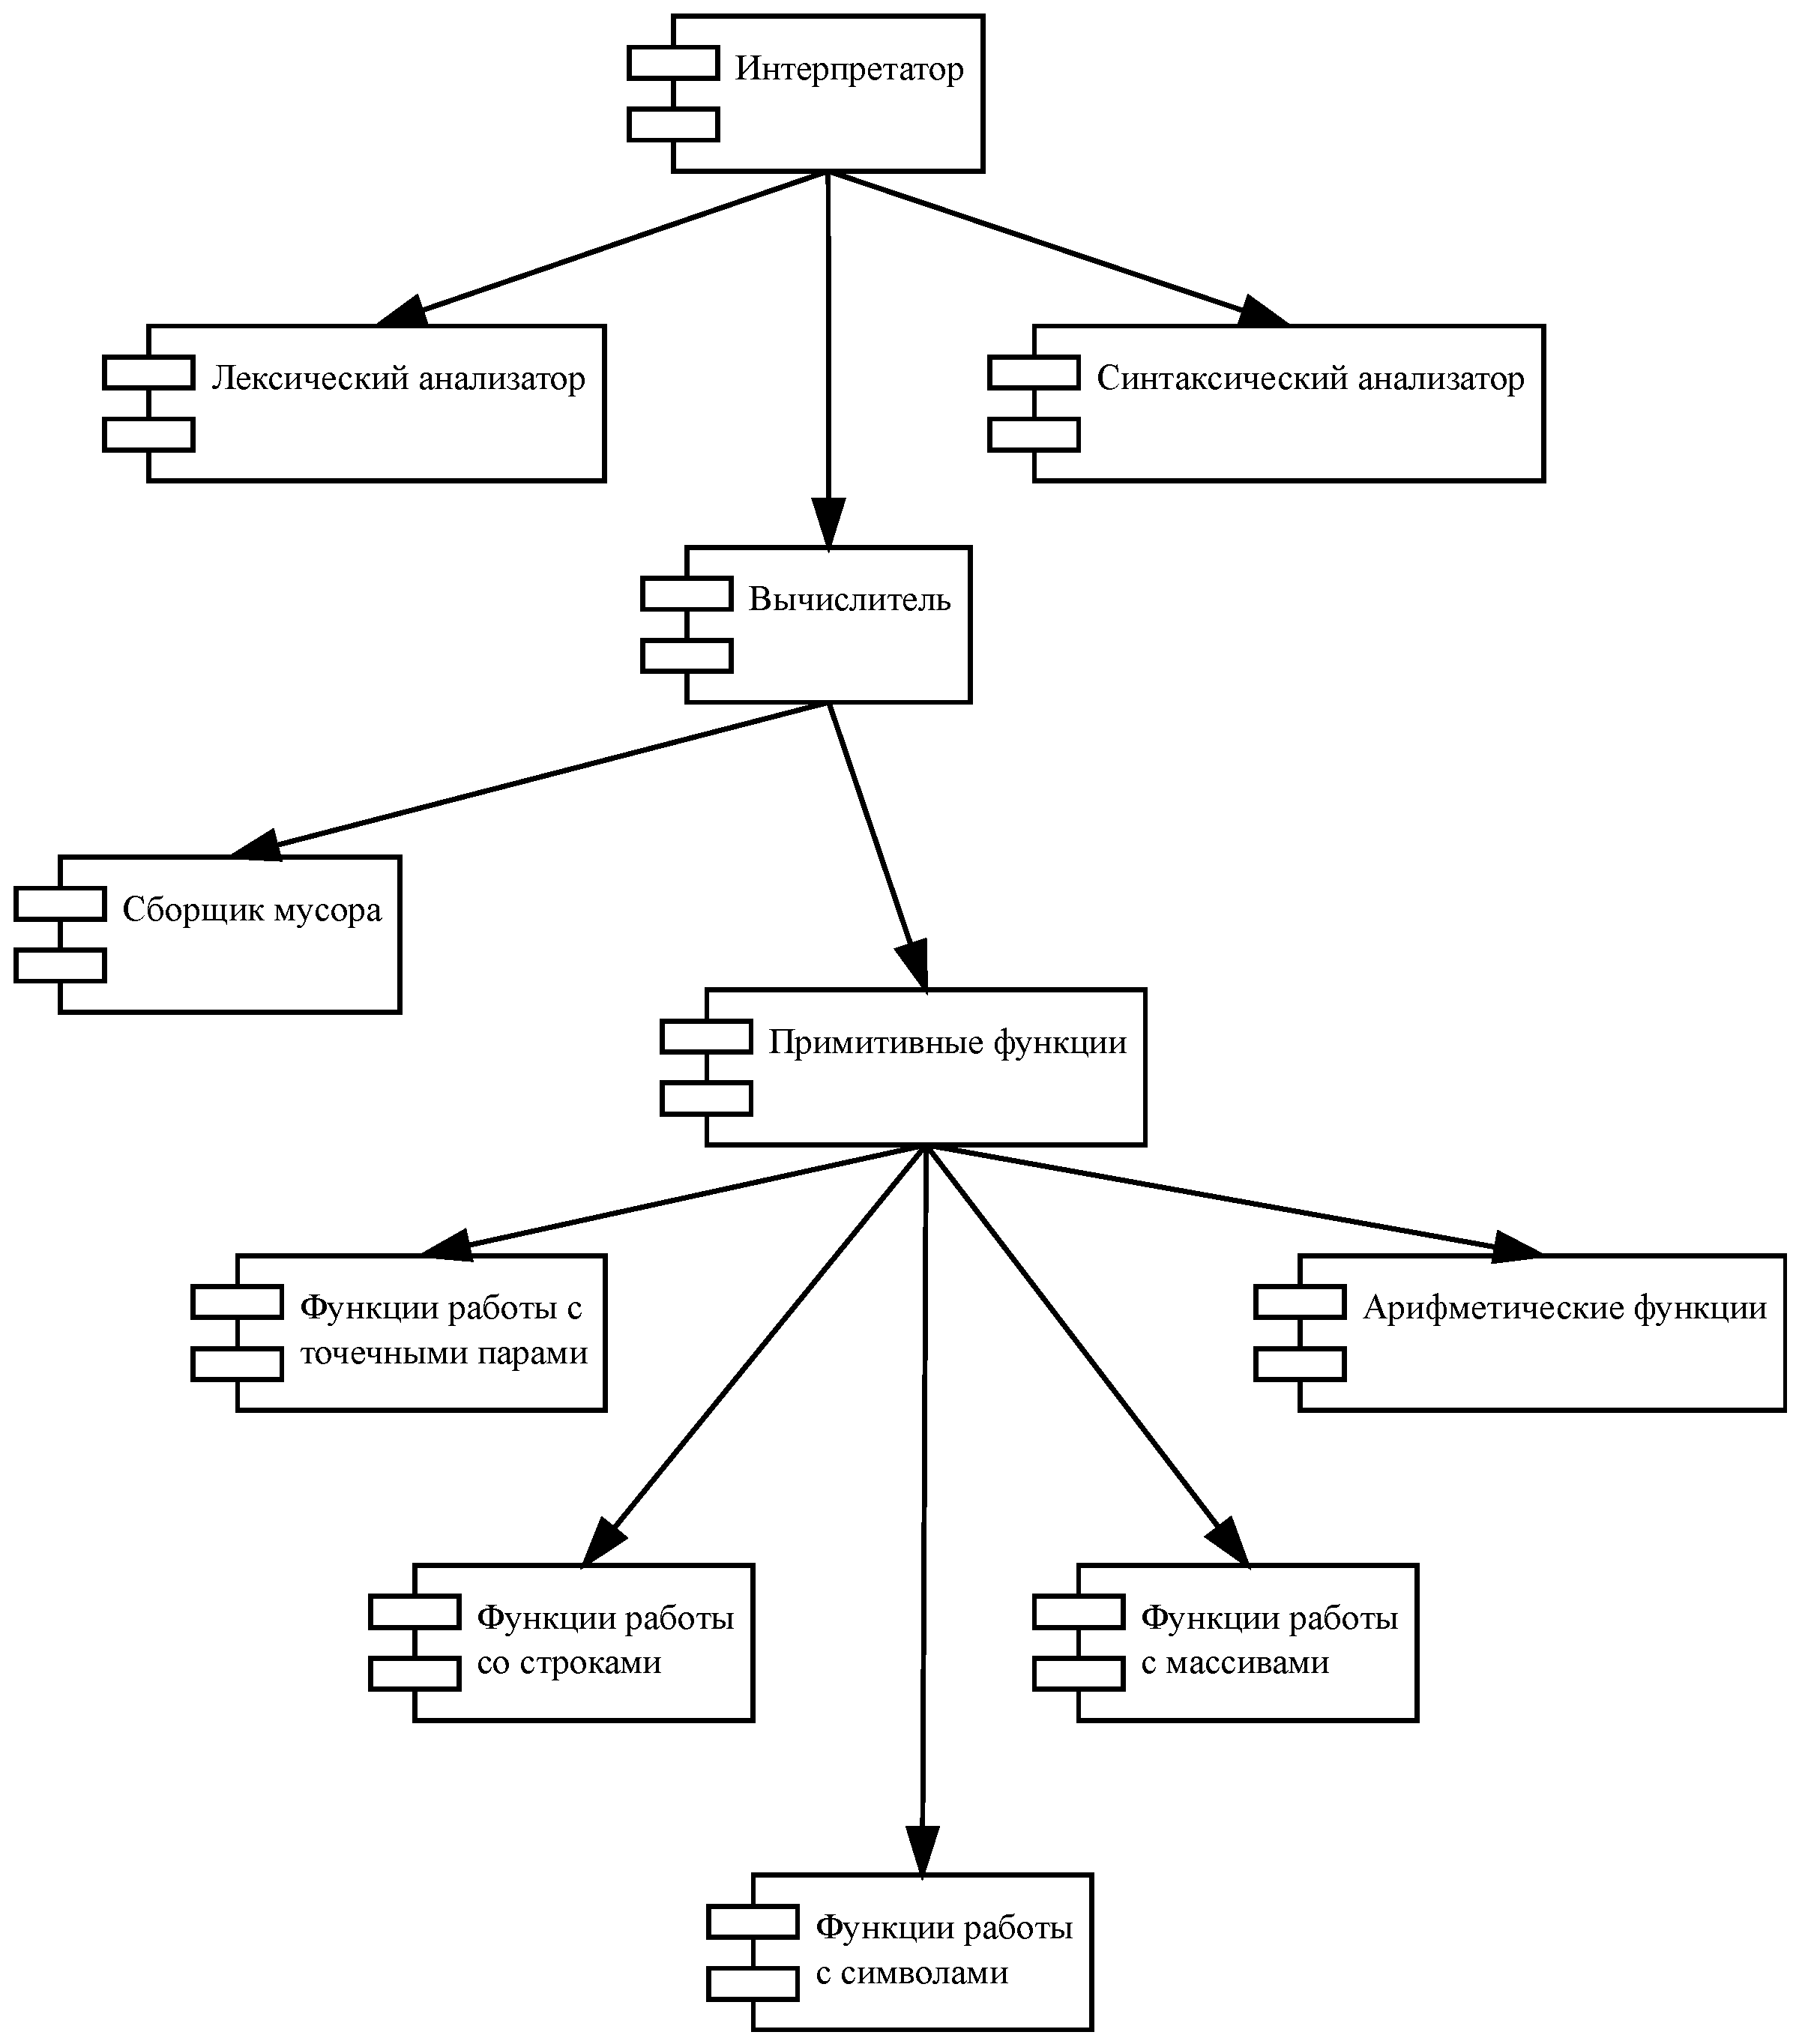
\includegraphics[width=1\linewidth]{kompdiagram}}
	\caption{Диаграмма компонентов интерпретатора}
	\label{kompdiagram:image}
\end{figure}

На рисунке \ref{kompdiagram:image} в виде UML-диаграммы показаны компоненты, составляющие интерпретатор.



\subsubsection{Алгоритм взаимодействия компонентов}
Пошаговый алгоритм взаимодействия компонентов, составляющих интерпретатор:

Шаг 1. Инициализируем исполнитель и регистрируем все примитивные функции ДЯП;

Шаг 2. Сохраняем текущее состояние программы, сохранив регистры процессора и стек с помощью setjmp. Если во время работы интерпретатора произойдёт ошибка - вывести на экран сообщение об ошибке и перейти к шагу 8;

Шаг 3. Запускаем синтаксический анализатор;

Шаг 4. Синтаксический анализатор вызывает лексический анализатор;

Шаг 5. Лексический анализатор на основе символов из входного потока формирует лексему и возвращает её;

Шаг 6. Синтаксический анализатор на основе полученной лексемы формирует объект для внутреннего представления и возвращает его;

Шаг 7. Если был достигнут конец входного потока - переходим к следующему шагу, иначе к шагу 12;

Шаг 8. Восстановить состояние программы к тому, что было сохранено на шаге 2, и перейти к шагу 13;

Шаг 9. Исполнитель производит вычисления с объектом, сформированным СА, в качестве аргумента и возвращает результат вычислений в виде объекта;

Шаг 10. Вывести возвращённый исполнителем объект на экран;

Шаг 11. Перейти к шагу 2;

Шаг 12. Сборщик мусора освобождает неиспользуемые объекты внутреннего представления. Перейти к шагу 2;

Шаг 13. Завершить работу интерпретатора.

\subsubsection{Лексический анализатор}
В разработанной программной системе лексический анализатор представляет собой компонент, в задачи которого входит считывание лексемы, проверка её на соответствие алфавиту языка и формирование токена.

Как только лексема была считана, она помещается в буфер размерностью в восемь символов.

Считанная лексема сравнивается со множеством зарезервированных под конструкции языка символов. При совпадении с каким-либо, формируется токен и ЛА возвращает его.


Сформированный токен представляет собой структуру с такими полями:
\begin{enumerate}
	\item type - тип токена;
	\item value - поле для токенов числового типа, содержит значение числа;
	\item str - поле для токенов строкового типа, значение строки.
\end{enumerate}

Особым случаем является считывание строки. Как только обнаруживается символ кавычки, запускается функция, собирающая символы до тех пор, пока:
\begin{itemize}
	\item не встретит второй символ кавычки, чем будет закончено считывание строки, после чего ЛА вернёт сформированный токен;
	\item количество символов не превысит допустимую длину строки, что приведёт к ошибке;
	\item не будет достигнут конец входного потока, что также приведёт к ошибке.
\end{itemize}


Если символ не является одним из зарезервированных, производится проверка на то, является он числом или символом.

Ввиду того, что имя символа, как и отрицательное число, может начинаться со знака минус решается неоднозначность, связанная с восприятием лексическим анализатором следующих символов. Для этого считывается ещё один символ и, если он является числовым, дальнейшая запись определяется как число, иначе как символ.

Если имя символа состоит из допустимых знаков, то бишь из алфавита языка, формируется токен типа символ и возвращается как результат работы ЛА. В противном случае, выдаётся ошибка о некорректности символа.

\subsubsection{Синтаксический анализатор}
Синтаксический анализатор запрашивает у ЛА по одному токену, строит для них внутреннее представление и повторяет процесс, пока не будет сформировано одно s-выражение, затем происходит возврат выражения.

СА, как и ЛА, выполняет проверку на ошибки, но уже синтаксические. Он выявляет отсутствие аргументов у операторов цитирования и квазицитирования, неоконченность списков (отсутствие закрывающей скобки) и отсутствие списка после символа '\#' для создания массива.


\subsubsection{Объекты внутреннего представления}
Как уже было рассмотрено ранее, весь программный код, считываемый из потока ввода, ещё на этапе обработки лексическим анализатором преобразуется в особые структуры, а не хранится в виде текста, ввиду необходимости манипулирования предоставленной им информацией, что было бы проблематичным и неэффективным при текстовом хранении. После обработки синтаксическим анализатором, все данные, полученные из программного кода, принимают своё окончательное представление и при исполнении инструкций меняется уже не их представление, а содержимое.

В разрабатываемом интерпретаторе все данные хранятся в виде структур языка C. Всего было разработано пять структур. Структура верхнего уровня object\_t, которая далее будет называться оболочкой объекта, является результатом выполнения любого s-выражения и доступ из примитивных функций к другим структурам осуществляется через поля этой структуры. Оставшиеся структуры реализуют четыре типа данных, за исключением числового: пара, символ, строка, массив.

Оболочка объекта позволяет узнать тип хранимых объектом данных, чтобы другие функции могли верно его обработать. Из поля объединения, соответствующего типу данных, функции будут получать число при числовом типе объекта или указатель на экземпляр другой структуры. Также оболочка содержит поля, обеспечивающие работу сборщика мусора. Её полная структура представлена в таблице \ref{strobjsh:table}.

\begin{xltabular}{\textwidth}{|l|l|p{5.7cm}|X|}
	\caption{Структура object\_t для оболочки объекта\label{strobjsh:table}}\\ \hline
	\centrow Имя & \centrow Тип & \centrow Описание & \centrow Возможные значения \\ \hline
	%\thead{1} & \thead{2} & \centrow 3 & \centrow 4 \\ \hline
	%\endfirsthead
	%\continuecaption{Продолжение таблицы \ref{strobjsh:table}}
	%\thead{1} & \thead{2} & \centrow 3 & \centrow 4 \\ \hline
	\finishhead
	type & type\_t & Тип объекта & NUMBER, SYMBOL, PAIR, STRING, ARRAY \\ \hline 
	u & union & Объединение, хранящее данные объекта в соответствии с его типом & Нет ограничений \\ \hline 
	next & object\_t* & Указатель для сборщика мусора на следующий свободный объект & Если NULL — данный объект является последним в списке свободных или список пуст, иначе содержит указатель на следующий свободный объект. \\ \hline 
	mark & int & Указывает на то, связан ли объект с символом.  & Если 1 — связан, 0 — не связан. \\ \hline 
	free & int & Свободен ли элемент для перезаписи. & Если 1 — элемент в списке свободных объектов, иначе занят
\end{xltabular}

Объединение u — используется для хранения значения, соответствующего объекту, в структуру которого включено это объединение. В зависимости от типа объекта, одно из полей symbol, pair, str, arr этого объединения будет иметь значение, остальные не используются. Структура этого объединения представлена в таблице \ref{strobjval:table}.

Для элемента value тип объекта - NUMBER, symbol — SYMBOL, pair — PAIR, str — STRING, arr — ARRAY.


\begin{xltabular}{\textwidth}{|c|c|X|}
	\caption{Структура u для хранения значения объекта\label{strobjval:table}}\\ \hline
	Имя  & \centrow  Тип & \centrow Описание \\ \hline
	%\endfirsthead
	%\continuecaption{Продолжение таблицы \ref{strobjval:table}}
	%Имя & \centrow Тип & \centrow Описание \\ \hline 
	\finishhead
	value & 
	int & 
	Содержит числовое значение, если объект имеет тип NUMBER \\ \hline 
	symbol\_s*  & symbol & Указывает на объект-символ, если объект имеет тип SYMBOL \\ \hline 
	pair\_s* & pair & Указывает на объект-пару, если объект имеет тип PAIR \\ \hline 
	string\_s* & str & Указывает на объект-строку, если объект имеет тип STRING \\ \hline 
	array\_s* & arr & Указывает на объект-массив, если объект имеет тип ARRAY
\end{xltabular}

Структуры остальных четырёх типов объектов представлены в таблицах \ref{strobjpair:table} - \ref{strobjsym:table}.

\begin{xltabular}{\textwidth}{|l|l|p{5.7cm}|X|}
	\caption{Структура pair\_t для объекта-пары\label{strobjpair:table}}\\ \hline
	\centrow Имя & \centrow Тип & \centrow Описание & \centrow Возможные значения \\ \hline
	\thead{1} & \thead{2} & \centrow 3 & \centrow 4 \\ \hline
	\endfirsthead
	\continuecaption{Продолжение таблицы \ref{strobjpair:table}}
	\thead{1} & \thead{2} & \centrow 3 & \centrow 4 \\ \hline
	\finishhead
	left & object\_t* & Указатель на левый элемент пары & Указатель на объект или NULL \\ \hline 
	right & object\_t* & Указатель на правый элемент пары & Указатель на объект или NULL \\ \hline 
	next & object\_t* & Указатель для сборщика мусора на следующий свободный объект-пару & Если NULL — данная пара является последней в списке свободных или список пуст, иначе содержит указатель на следующий свободный объект-пару. \\ \hline 
	free & int & Свободна ли пара для перезаписи  & Если 1 — пара в списке свободных пар, иначе занята
\end{xltabular}

\begin{xltabular}{\textwidth}{|l|l|p{5.7cm}|X|}
	\caption{Структура string\_t для объекта-строки\label{strobjstr:table}}\\ \hline
	\centrow Имя & \centrow Тип & \centrow Описание & \centrow Возможные значения \\ \hline
	%\thead{1} & \thead{2} & \centrow 3 & \centrow 4 \\ \hline
	%\endfirsthead
	%\continuecaption{Продолжение таблицы \ref{strobjstr:table}}
	%\thead{1} & \thead{2} & \centrow 3 & \centrow 4 \\ \hline
	\finishhead
	data & char* & Данные строки & Нет ограничений \\ \hline 
	length & int & Длина строки & Натуральное число, соответствующее количеству символов в строке \\ \hline 
	next & string\_t* & Указатель для сборщика мусора на следующую свободную строковый объект & Если NULL — данная строка является последней в списке свободных или список пуст, иначе содержит указатель на следующую свободную объект-пару. \\ \hline 
	free & int & Свободна ли строка для перезаписи & Если 1 — строка в списке свободных строк, иначе занята
\end{xltabular}


\begin{xltabular}{\textwidth}{|l|l|p{5.7cm}|X|}
	\caption{Структура array\_t для объекта-массива\label{strobjarr:table}}\\ \hline
	\centrow Имя & \centrow Тип & \centrow Описание & \centrow Возможные значения \\ \hline
	\thead{1} & \thead{2} & \centrow 3 & \centrow 4 \\ \hline
	\endfirsthead
	\continuecaption{Продолжение таблицы \ref{strobjarr:table}}
	\thead{1} & \thead{2} & \centrow 3 & \centrow 4 \\ \hline
	\finishhead
	data & object\_t** & Данные массива & Нет ограничений \\ \hline 
	length & int & Количество элементов массива & Натуральное число, соответствующее количеству элементов массива \\ \hline 
	next & array\_t* & Указатель для сборщика мусора на следующий свободный массив & Если NULL — данный объект-массив является последним в списке свободных или список пуст, иначе содержит указатель на следующий свободный объект-массив. \\ \hline 
	free & int & Свободен ли массив для перезаписи & Если 1 — массив в списке свободных массивов, иначе занят
\end{xltabular}

\begin{xltabular}{\textwidth}{|l|l|p{5.7cm}|X|}
	\caption{Структура symbol\_t для объекта-символа\label{strobjsym:table}}\\ \hline
	\centrow Имя & \centrow Тип & \centrow Описание & \centrow Возможные значения \\ \hline
	\thead{1} & \thead{2} & \centrow 3 & \centrow 4 \\ \hline
	\endfirsthead
	\continuecaption{Продолжение таблицы \ref{strobjsym:table}}
	\thead{1} & \thead{2} & \centrow 3 & \centrow 4 \\ \hline
	\finishhead
	str & char[] & Имя символа & NUMBER \\ \hline 
	next & symbol\_t* & Указатель на следующий за данным символ в хеш-таблице & Нет ограничений \\ \hline 
	value & object\_t * & Указатель на объект, связанный с символом & Если NULL — данный объект является последним в списке свободных или список пуст, иначе содержит указатель на следующий свободный объект. \\ \hline 
	lambda & object\_t* & Указатель на объект лямбда-выражения, связанный с символом & Если 1 — связан, 0 — не связан. \\ \hline
	func & func\_t & Указатель на примитив функции, связанный с символом. & Нет ограничений
\end{xltabular}


\subsubsection{Исполнитель}

Алгоритм работы исполнителя представлен пошагово, где некоторые шаги имеют подшаги, которые также надо пройти, если условие верхнего уровня выполняется:

Шаг 1. Если obj равно NULL, вернуть NULL, окончив этим выполнение алгоритма;

Шаг 2. Иначе, если тип obj равен NUMBER, STRING или ARRAY - вернуть obj, окончив этим выполнение алгоритма;

Шаг 3. Иначе, если тип obj равен SYMBOL;

Подшаг 3.1. Если в env есть объект, содержащий указатель на искомый символ, вернуть этот объект, окончив этим выполнение алгоритма;

Подшаг 3.2. Иначе проверить наличие символа, соответствующего имени искомого, в хеш-таблице. Если символ найден и ссылается на объект, содержащий его, вернуть данный объект, окончив этим выполнение алгоритма;

Подшаг 3.3. Иначе вывести на экран ошибку, оповещающую об отсутствии символа: "Unknown SYMBOL: <имя символа>", а также вернуть значение, оповещающее об ошибке - ERROR, окончив этим выполнение алгоритма;

Шаг 4. Иначе, если тип obj равен PAIR;

Подшаг 4.1. Если первый элемент цепи obj является цепью;

Подшаг 4.1.1. Если первый элемент цепи obj имеет особенности, указывающие на то, что он является лямбда-выражением - выполнить это лямбда-выражение в окружении env и вернуть результат, окончив этим выполнение алгоритма;

Подшаг 4.1.2. Иначе вернуть ERROR;

Подшаг 4.2. Ввести переменную s. Найти (или создать при отсутствии), символ в хеш-таблице, имя которого соответствует имени искомого, и задать значением для s этот символ; Ввести переменную args;

Подшаг 4.3. Если первый элемент цепи obj имеет особенности, позволяющие определить его как специальную форму, задать для args значение хвоста цепи obj;

Подшаг 4.4. Иначе рекурсивно вычислить в окружении env список аргументов из хвоста цепи obj;

Подшаг 4.5. Если args равно ERROR - вывести на экран ошибку, сообщающую об ошибке в аргументах и сами аргументы, после чего вернуть ERROR, окончив этим выполнение алгоритма;

Подшаг 4.6. Если символ s содержит указатель на функцию - выполнить её с аргументами args в окружении env и вернуть вычисленное значение, окончив этим выполнение алгоритма;

Подшаг 4.7. Иначе, если символ s содержит указатель на функцию примитивного типа - выполнить её с аргументами args и вернуть вычисленное значение, окончив этим выполнение алгоритма;

Подшаг 4.8. Иначе, если символ s содержит указатель на макрос - вычислить макро-подстановку с аргументами args в окружении env и вернуть вычисленное значение, окончив этим выполнение алгоритма;

Подшаг 4.9. Иначе вывести на экран сообщение об ошибке, сообщающее о том, что функцию не удалось найти, после чего вернуть ERROR, окончив этим выполнение алгоритма;

Шаг 5. Иначе вывести на экран ошибку, сообщающую о том, что исполнитель не может определить тип переданного ему объекта. Конец алгоритма.

\subsubsection{Сборщик мусора}
Разработанный в рамках этой работы сборщик мусора работает в две фазы по алгоритму пометки и очистки и осуществляет сборку по следующему принципу.
Объекты и пары освобождаются в конце вычисления выражения верхнего уровня. Символы сборщиком не затрагиваются.

\begin{enumerate}
	\item Фаза пометки.
	Обходим все символы в таблице символов и выполняем пометку объектов, на которые они указывают. Пометка реализуется через поле mark в структуре объекта и пары. Если помечается объект-пара, то левый и правый объекты этой пары пометятся рекурсивно.
	
	\item Фаза очистки.
	Обходим все выделенные объекты и пары. Если есть пометка - снимаем её, иначе рекурсивно освобождаем объект и/или пару.
	
\end{enumerate}

\subsubsection{Примитивные функции}

Было реализовано множество функций, встроенных в разрабатываемый язык.

\paragraph{Арифметические функции}

Разработанные арифметические функции позволяют выполнять базовые арифметические операции вроде суммирования и деления, а также побитовые, эквивалентности и сравнения. Перечень таких функций, их описания и примеры использования представлены в таблице \ref{funcprimarith:table}.

Также там содержатся перечни типов обрабатываемых функцией аргументов. Перечисление происходит через запятую, если функция принимает сразу несколько аргументов. Если же необходимо указать что для одного аргумента функция может принимать объекты определённых нескольких типов, они записываются через "или".

\begin{xltabular}{\textwidth}{|p{3.6cm}|p{2cm}|p{6cm}|X|}
	\caption{Перечень функций арифметического модуля\label{funcprimarith:table}}\\ \hline
	\centrow Имя & \centrow Аргу- \linebreak менты & \centrow Описание & \centrow Пример \\ \hline
	\thead{1} & \thead{2} & \centrow 3 & \centrow 4 \\ \hline
	\endfirsthead
	\continuecaption{Продолжение таблицы \ref{funcprimarith:table}}
	\thead{1} & \thead{2} & \centrow 3 & \centrow 4 \\ \hline
	\finishhead
	Суммирование & Числа & Возвращает сумму чисел списка & < (+ 1 2 3) \linebreak > 6 \\ \hline 
	Вычитание & Числа & Возвращает разность чисел списка & < (- 5 2 1) \linebreak > 2 \\ \hline 
	Произведение & Числа & Возвращает произведение чисел списка & < (* 2 1 2) \linebreak 4 \\ \hline 
	Деление & Числа & Возвращает результат от деления чисел списка & < (/ 8 2) \linebreak 4 \\ \hline 
	Больше чем & Числа & Возвращает результат сравнения на большее из двух чисел списка. Если левое больше правого - T, иначе NIL & < (> 2 1) \linebreak > T \\ \hline 
	Меньше чем & Числа & Возвращает результат сравнения на меньшее из двух чисел списка. Если левое меньше правого - T, иначе NIL & < (< 2 1) \linebreak > NIL \\ \hline 
	Разность чисел & Числа & Возвращает результат сравнения на меньшее из двух чисел списка. Если числа равны - T, иначе NIL & < (= 2 1) \linebreak > NIL \\ \hline 
	Эквивалентность объектов по значению & Любые & Возвращает результат сравнения значений двух объектов списка. Если значения идентичны - T, иначе NIL & < (equal 2 2) \linebreak > T \\ \hline 
	Побитовое И & Числа & Возвращает результат побитового умножения чисел списка & < (\& 1 1 0) \linebreak > 0 \\ \hline 
	Побитовое ИЛИ & Числа & Возвращает результат побитового сложения чисел списка & < (bitor 1 1 0) \linebreak > 0 \\ \hline 
	Побитовый сдвиг влево & Числа & Первый аргумент - число, на которое будет применён сдвиг, второй - число бит сдвига. Возвращает результат побитового сдвига влево числа & < (<< 1 2) \linebreak > 8 \\ \hline 
	Побитовый сдвиг вправо & Числа & Первый аргумент - число, на которое будет применён сдвиг, второй - число бит сдвига. Возвращает результат побитового сдвига вправо числа & < (>> 0xF0 8) \linebreak > 15
\end{xltabular}

\paragraph{Функции исполнителя}

Исполнитель содержит в своём модуле все функции, отвечающие за:
\begin{itemize}
	\item объявление функций, переменных, макросов и их вычисление нестандартными способами;
	\item логические операторы;
	\item создание списков;
	\item цитирование и квазицитирование;
	\item проверка объектов на атомарность и эквивалентность атомов.
\end{itemize}

Полный перечень функций представлен в таблице \ref{funcprimeval:table}.

\begin{xltabular}{\textwidth}{|p{3.6cm}|p{1.8cm}|p{6cm}|X|}
	\caption{Перечень функций исполнительного модуля\label{funcprimeval:table}}\\ \hline
	\centrow Имя & \centrow Аргу- \linebreak менты & \centrow Описание & \centrow Пример \\ \hline
	\thead{1} & \thead{2} & \centrow 3 & \centrow 4 \\ \hline
	\endfirsthead
	\continuecaption{Продолжение таблицы \ref{funcprimeval:table}}
	\thead{1} & \thead{2} & \centrow 3 & \centrow 4 \\ \hline
	\finishhead
	Проверка на атом & Любой & Если объект является атомом - возвращает T, иначе NIL & < (atom 'a) \linebreak > T \\ \hline 
	Эквивалентность атомов & Любые & Если два атома равны - возвращает T, иначе NIL & < (eq 'a 'a) \linebreak > T \\ \hline 
	Цитирование & Любой & Возвращает аргумент без вычисления & < (quote (+ 1 2)) \linebreak > (+ 1 2) \\ \hline 
	Квазицитирова-\linebreak ние & Любой & Возвращает аргумент с частичными вычислениями & < (setq b 1) \linebreak < (backquote (+ ,b 2 3)) \linebreak > (+ 1 2 3) \\ \hline 
	Условие & Списки & Аргументы вычисляются до тех пор, пока не будет достигнут результат вычисления T. Каждый аргумент - список, где первый элемент - проверяемое выражение, а второй - результат, который будет возвращен при истинности выражения & < (cond ((eq 'a 'b) 1) (t 2)) \linebreak > 2 \\ \hline 
	Объявление функции & Символ, списки & Объявляет новую функцию с именем, соответствующим первому аргументу, списку параметров - второму аргументу и телу функции - третьему & < (defun pl (x) (+ 1 x)) \linebreak < (pl 2) \linebreak > 3 \\ \hline 
	Применение функции к аргументам & Символ или лямбда-выра- \linebreak жение, любые & Эта функция применяет значение первого аргумента как функцию к остальным аргументам и возвращает результат применения & < (funcall '+ 1 2) \linebreak > 3 \\ \hline 
	Объявление макроса & Символ, списки & Объявляет новый макрос с именем, соответствующим первому аргументу, списку параметров - второму аргументу и телу макроса - третьему & < (defmacro db (x) `(* 2 ,x)) \linebreak < (db 3) \linebreak > 6 \\ \hline 
	Макроподста-\linebreak новка & Список & Возвращает результат макроподстановки для переданного в качестве аргумента квотированного вызова макроса & < (defmacro db (x) `(* 2 ,x)) \linebreak < (macroexpand '(db 3)) \linebreak > (* 2 3) \\ \hline 
	Последова-\linebreak тельное выполнение & Любые & Последовательно вычисляет все s-выражения, переданные в качестве аргументов, и возвращает результат последнего вычисленного & < (progn  (+ 1 2) 5) \linebreak > 5 \\ \hline 
	Объявление переменной & Символ, любой & Объявляет переменную с именем, переданным в качестве первого аргумента, и значением - второго. & < (setq val 3) \linebreak > 3 \\ \hline 
	Логическое ИЛИ & Списки & Возвращает T после нахождения первого истинного условия. Если истинных нет - вернёт NIL. Должно быть хотя бы одно условие & < (or (= 1 2)) \linebreak > NIL \\ \hline 
	Логическое И & Списки & Возвращает NIL после нахождения первого ложного условия. Если ложных нет - вернёт T. Должно быть хотя бы одно условие & < (or (= 1 2)) \linebreak > NIL \\ \hline 
	Создание списка & Любые & Возвращает список, сформированный из переданных аргументов & < (list 1 'x '(12 3)) \linebreak > (1 X (12 3)) \\ \hline 
	Вычисление s-выражения & Любой & Вычисляет s-выражение и возвращает результат его вычисления & < (eval '(/ 4 2)) \linebreak > 2 \\ \hline 
\end{xltabular}

\paragraph{Функции модуля работы с массивами}

Этот модуль функций включает инструменты для создания массива, получения и установки значения.

Полный перечень функций представлен в таблице \ref{funcprimarr:table}.

\begin{xltabular}{\textwidth}{|p{3.6cm}|p{1.8cm}|p{6cm}|X|}
	\caption{Перечень функций модуля работы с массивами\label{funcprimarr:table}}\\ \hline
	\centrow Имя & \centrow Аргу- \linebreak менты & \centrow Описание & \centrow Пример \\ \hline
	%\thead{1} & \thead{2} & \centrow 3 & \centrow 4 \\ \hline
	%\endfirsthead
	%\continuecaption{Продолжение таблицы \ref{funcprimarr:table}}
	%\thead{1} & \thead{2} & \centrow 3 & \centrow 4 \\ \hline
	\finishhead
	Создание пустого массива & Число & Создает пустой массив заданной аргументом длины и возвращает его & < (make-array 3) \linebreak > \#(NIL NIL NIL) \\ \hline 
	Задать значение элементу & Массив, число, любой & Задает значение элементу массива с некоторым индексом и возвращает массив. Аргументы: массив, индекс, значение & < (seta \#(1 2) 0 10)) \linebreak > \#(10 2) \\ \hline 
	Чтение элемента & Массив, число & Возвращает значение элемента массива по некоторому индексу. Аргументы: массив, индекс & < (aref \#(4 2) 1) \linebreak > 2 \\ \hline 
	
\end{xltabular}

\paragraph{Функции модуля работы с точечными парами}

Этот модуль реализует инструменты для работы со списками и точечными парами.

Полный перечень функций представлен в таблице \ref{funcprimpair:table}.

\begin{xltabular}{\textwidth}{|p{3.6cm}|p{1.8cm}|p{6cm}|X|}
	\caption{Перечень функций модуля работы с точечными парами\label{funcprimpair:table}}\\ \hline
	\centrow Имя & \centrow Аргу- \linebreak менты & \centrow Описание & \centrow Пример \\ \hline
	\thead{1} & \thead{2} & \centrow 3 & \centrow 4 \\ \hline
	\endfirsthead
	\continuecaption{Продолжение таблицы \ref{funcprimpair:table}}
	\thead{1} & \thead{2} & \centrow 3 & \centrow 4 \\ \hline
	\finishhead
	Первый элемент & Список & Возвращает первый элемент переданного аргументом списка & < (car '(a b)) \linebreak > A \\ \hline 
	Исключение первого элемента & Список & Возвращает переданный аргументом список без первого элемента & < (cdr '(a b c)) \linebreak > B C \\ \hline 
	Создание пары & Список & Создаёт точечную пару, где левая часть - первый элемент переданного аргументом списка, правая - второй. & < (cons 'a 'b) \linebreak > (A . B) \\ \hline 
	Заменить левую часть пары & Пара, любой & Заменяет левую часть пары, переданной первым аргументом, значением второго аргумента и возвращает получившуюся пару & < (rplaca '(a . b) 'd) \linebreak > (D . B) \\ \hline 
	Заменить правую часть пары & Пара, любой & Заменяет правую часть пары, переданной первым аргументом, значением второго аргумента и возвращает получившуюся пару & < (rplacd '(a . b) 'd) \linebreak > (A . D)
	
\end{xltabular}

\paragraph{Функции модуля работы со строками}

Этот модуль реализует инструменты для работы непосредственно со строками и строковыми преобразованиями, а также с именами символов

Полный перечень функций представлен в таблице \ref{funcprimstr:table}.

\begin{xltabular}{\textwidth}{|p{3.6cm}|p{1.8cm}|p{6cm}|X|}
	\caption{Перечень функций модуля работы со строками\label{funcprimstr:table}}\\ \hline
	\centrow Имя & \centrow Аргу- \linebreak менты & \centrow Описание & \centrow Пример \\ \hline
	\thead{1} & \thead{2} & \centrow 3 & \centrow 4 \\ \hline
	\endfirsthead
	\continuecaption{Продолжение таблицы \ref{funcprimstr:table}}
	\thead{1} & \thead{2} & \centrow 3 & \centrow 4 \\ \hline
	\finishhead
	Создание символа & Строка & Создаёт символ с именем, соответствующим первому аргументу, и возвращает созданный символ & < (intern "A") \linebreak > A \\ \hline 
	Объединение двух строк & Строка, строка & Возвращает объединение двух строк, переданных аргументами & < (concat "a" "\_") \linebreak > "a\_" \\ \hline 
	Получение имени символа & Символ & Возвращает имя символа, переданного в качестве аргумента & < (symbol-name 'sym) \linebreak > SYM \\ \hline 
	Получение длины строки & Строка & Возвращает длину строки, переданной в качестве аргумента & < (string-size "123") \linebreak > 3 \\ \hline 
	Получение символа из строки & Строка, число & Возвращает код символа из строки по некоторому индексу & < (char "123" 2) \linebreak > 51 \\ \hline 
	Получение подстроки & Строка, число, число & Возвращает подстроку из строки, начиная с начального индекса и по конечный индекс, не включая последний. Аргументы: строка начальный\_индекс конечный\_индекс & < (subseq "123" 0 2) \linebreak > "12" \\ \hline 
	Число в строку & Число & Возвращает строку, содержащую число, переданное в качестве аргумента & < (inttostr 12) \linebreak > "12" \\ \hline 
	Код символа в строку & Число & Возвращает символ в строковом представлении на основе кода символа, переданного в качестве аргумента & < (code-char 51) \linebreak > 3
	
\end{xltabular}
\ifПрактика{}\else{
   \section{Рабочий проект}

\subsection{Модули, разработанные для реализации интерпретатора}

С целью обеспечить логическое разделение кода, во время его написания были разработаны модули, представляющие собой связанные друг с другом исходные файлы на языке C, составляющие функциональность интерпретатора.


\begin{figure}[h!t]
	\center{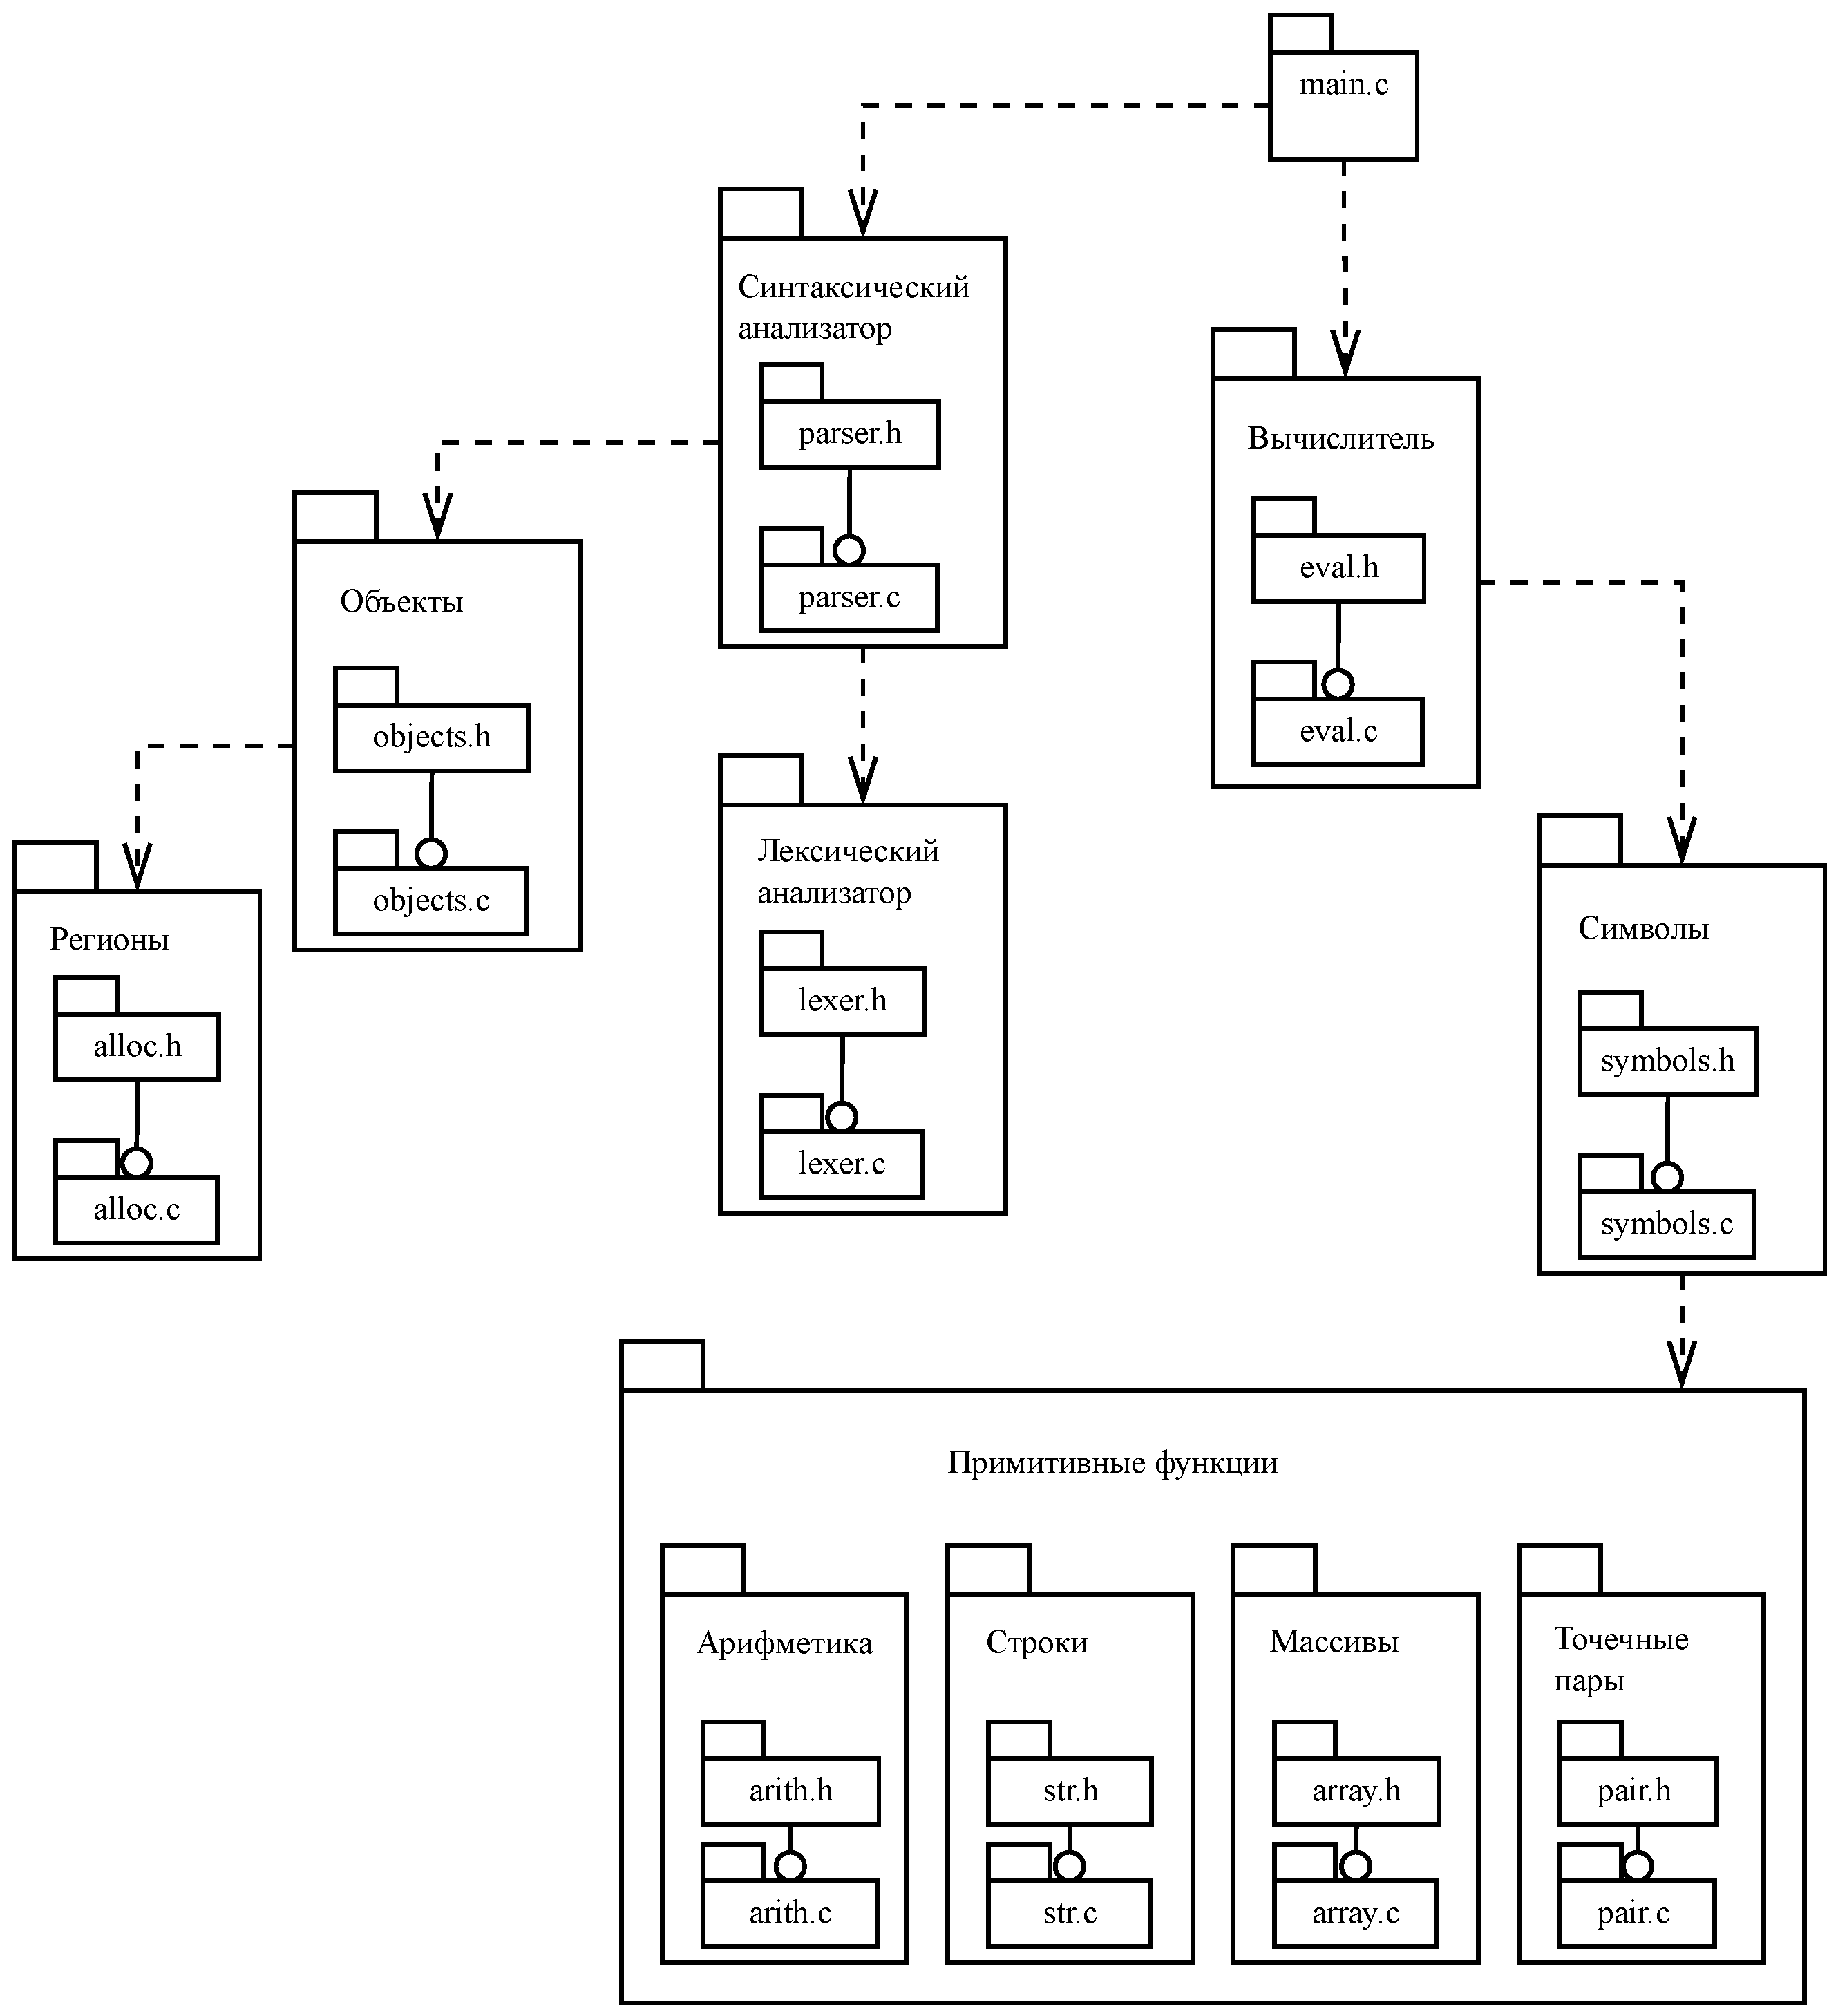
\includegraphics[width=1\linewidth]{uml_package}}
	\caption{Диаграмма пакетов интерпретатора}
	\label{uml_package:image}
\end{figure}

Эти файлы и их зависимость друг от друга продемонстрированы на рисунке \ref{uml_package:image} в виде UML-диаграммы пакетов \cite{e32}.

Перечень модулей представлен в таблице \ref{modules:table}, куда входят их имена, роль в структуре разрабатываемой ПС, а также описания выполняемых ими задач.

\begin{xltabular}{\textwidth}{|l|p{4cm}|X|}
	\caption{Модули интерпретатора\label{modules:table}} \\ \hline
	\centrow Имя & \centrow Роль & \centrow Задача \\ \hline
	\thead{1} & \thead{2} & \centrow 3 \\ \hline
	\endfirsthead
	\continuecaption{Продолжение таблицы \ref{modules:table}}
	\thead{1} & \thead{2} & \centrow 3 \\ \hline
	\finishhead
	main.c & Главный модуль & Выполняет инициализацию всех остальных модулей, организует работу между ЛА и исполнителем, запускает сборщик мусора, выполняет возвращение в точку до ошибки при её возникновении \\ \hline
	alloc.c & Модуль работы с регионами & Хранение массивов и строк реализовано через \quotes{регионы}, инструменты для управления которыми помещены в этот модуль \\ \hline
	objects.c & Модуль внутреннего объектного представления & Содержит функции, позволяющие создавать объекты и манипулировать ими \\ \hline
	arith.c & Модуль арифметических функций & Реализует примитивные арифметические функции \\ \hline
	str.c & Модуль работы со строками & Реализует инструменты для создания объектов-строк и манипуляции ими \\ \hline
	array.c & Модуль работы с массивами & Реализует инструменты для создания объектов-массивов и манипуляции ими \\ \hline
	symbols.c & Модуль работы с символами & Реализует инструменты для создания объектов-символов и манипуляции ими \\ \hline
	pair.c & Модуль работы с парами & Реализует инструменты для создания точечных пар и списков и манипуляции ими \\ \hline
	lexer.c & Лексический анализатор & Реализует все возможности, необходимые для анализа лексем и создания токенов на их основе \\ \hline
	parser.c & Синтаксический анализатор & Реализует все возможности, необходимые для формирования объектов внутреннего представления на основе токенов \\ \hline
	eval.c & Модуль исполнения & Исполняет s-выражения, связывая тем самым примитивные функции языка и объекты внутреннего представления \\ \hline
\end{xltabular}

\subsection{Спецификация модулей лексического и синтаксического анализаторов}

Для более глубокого раскрытия задач ЛА (lexer.c) и СА (parser.c) в таблицах \ref{modinfo_lexer_fields:table} - \ref{modinfo_parser_funcs:table} приведены поля и методы этих модулей с их именами, описаниями и типами входных и выходных данных.

\begin{xltabular}{\textwidth}{|l|p{3.5cm}|X|}
	\caption{Спецификация полей модуля \quotes{lexer.c}\label{modinfo_lexer_fields:table}}\\ \hline
	\centrow Имя & \centrow Тип & \centrow Описание \\ \hline
	\thead{1} & \thead{2} & \centrow 3 \\ \hline
	\endfirsthead
	\continuecaption{Продолжение таблицы \ref{modinfo_lexer_fields:table}}
	\thead{1} & \thead{2} & \centrow 3 \\ \hline
	\finishhead
	cur\_symbol & char & Символ, считанный последним (текущий символ) \\ \hline
	token & token\_t & Токен, генерируемый в момент лексического анализа (текущий токен) \\ \hline
	token\_error & int & Флаг, оповещающий парсер о возникновении ошибки при лексическом разборе. Если произошла ошибка, его значение -- 1, иначе 0 \\ \hline
	SYMBOL\_BUFFER\_SIZE & Целочисленная символическая константа & Задаёт размер буфера символов \\ \hline
	symbol\_buffer & char[] & Буфер символов, считанных из стандартного потока ввода. Имеет обратный порядок элементов. Размер буфера задаётся значением \quotes{SYMBOL\_BUFFER\_SIZE} \\ \hline
	buffer\_write\_pos & int & Текущая позиция записи в буфере символов \\ \hline
	buffer\_read\_pos & int & Текущая позиция чтения из буфера символов \\ \hline
\end{xltabular}

\begin{xltabular}{\textwidth}{|l|p{3.2cm}|X|}
	\caption{Спецификация методов модуля \quotes{lexer.c}\label{modinfo_lexer_funcs:table}}\\ \hline
	\centrow Имя & \centrow Ввод / вывод & \centrow Описание \\ \hline
	\thead{1} & \thead{2} & \centrow 3 \\ \hline
	\endfirsthead
	\continuecaption{Продолжение таблицы \ref{modinfo_lexer_funcs:table}}
	\thead{1} & \thead{2} & \centrow 3 \\ \hline
	\finishhead
	get\_cur\_char & > void & Считывает символ из потока ввода и помещает его в буфер. Когда буфер заполняется, производится сдвиг позиций чтения и записи \\ \hline
	unget\_cur\_char & > void & Возвращает позицию чтения назад на единицу и переприсваивает текущий символ \\ \hline
	is\_whitespace & < char c \linebreak > int & Проверяет является ли символ пробельным (пробел, перенос строки, табуляция) \\ \hline
	skip\_comment & > void & Пропускает все символы, пока не достигнет переноса строки или конца входного потока \\ \hline
	skip\_white\_space & > void & Выполняет пропуск при обнаружении пробельного символа или знака комментария, оперируя для этого функциями \quotes{is\_whitespace} \quotes{skip\_comment} \\ \hline
	is\_digit & < char c \linebreak > int & Проверяет является ли символ \quotes{c} цифрой (от 0 до 9). Если да -- возвращает 1, иначе 0 \\ \hline
	is\_alpha & < char c \linebreak > int & Проверяет является ли символ \quotes{c} буквой латинского алфавита в верхнем или нижнем регистре. Если да -- возвращает 1, иначе 0 \\ \hline
	is\_symbol & < char c \linebreak > int & Проверяет является ли символ \quotes{c} разрешённым (+-*/=\_\&|<>). Если да -- возвращает 1, иначе 0 \\ \hline
	is\_hex\_symbol & < char c \linebreak > int & Проверяет является ли символ \quotes{c} одним из шестнадцатеричных символов от \quotes{a} до \quotes{f} и от \quotes{A} до \quotes{F} \\ \hline
	is\_delimeter & < char c \linebreak > int & Проверяет является ли символ \quotes{c} разделителем: открывающая и закрывающая скобки, обратная косая черта, двойная кавычка, пробельный символ, конец потока \\ \hline
	hex\_num & > int & Преобразует шестнадцатеричное число из потока ввода в десятичное и возвращает его \\ \hline
	get\_float\_num & > void & Принимает целую часть \quotes{int\_num} от вещественного числа и считывает оставшиеся после точки числа. Преобразует имеющиеся данные в число с плавающей точкой в формате целочисленного (int) и возвращает его \\ \hline
	get\_num & > int & Считывает из потока ввода число в десятичной или шестнадцатеричной системе счисления и приводит его к десятичной. Записывает его в переменную \quotes{cur\_num}, после чего возвращает \\ \hline
	get\_symbol & < char *cur\_str \linebreak > void & Считывает имя символа из \quotes{cur\_str} и проверяет его на корректность. Если не корректное -- задаёт для \quotes{token\_error} значение 1 и выводит ошибку \\ \hline
	get\_string & < char *cur\_str \linebreak > void & Считывает строку, обрамлённую двойными кавычками, из \quotes{cur\_str}. Если отсутствует закрывающая кавычка, выводит ошибку и устанавливает значение \quotes{token\_error} в 1\\ \hline
	get\_comma & > token\_t & Обрабатывает лексему \quotes{,} или \quotes{,@} из входного потока, формирует для неё токен и возвращает его \\ \hline
	get\_sharp & > token\_t & Обрабатывает лексему \quotes{\#} или \quotes{\# \textbackslash} из входного потока, формирует для неё токен и возвращает его \\ \hline
	get\_token & > token\_t* & Считывает лексему из потока ввода, формирует на её основе токен и возвращает его, используя для этого все вышеперечисленные функции
	
\end{xltabular}

\begin{xltabular}{\textwidth}{|l|p{3.5cm}|X|}
	\caption{Спецификация полей модуля \quotes{parser.c}\label{modinfo_parser_fields:table}}\\ \hline
	\centrow Имя & \centrow Тип & \centrow Описание \\ \hline
	%\thead{1} & \thead{2} & \centrow 3 \\ \hline
	%\endfirsthead
	%\continuecaption{Продолжение таблицы \ref{modinfo_parser_fields:table}}
	%\thead{1} & \thead{2} & \centrow 3 \\ \hline
	\finishhead
	token\_error & extern int & Флаг, устанавливаемый лексером для оповещения парсера о возникновении ошибки при лексическом разборе. Если произошла ошибка, его значение -- 1, иначе 0 \\ \hline
	cur\_token & token\_t & Последний полученный токен (текущий токен)
\end{xltabular}

\begin{xltabular}{\textwidth}{|l|p{3.2cm}|X|}
	\caption{Спецификация методов модуля \quotes{parser.c}\label{modinfo_parser_funcs:table}}\\ \hline
	\centrow Имя & \centrow Ввод / вывод & \centrow Описание \\ \hline
	\thead{1} & \thead{2} & \centrow 3 \\ \hline
	\endfirsthead
	\continuecaption{Продолжение таблицы \ref{modinfo_parser_funcs:table}}
	\thead{1} & \thead{2} & \centrow 3 \\ \hline
	\finishhead
	strupr & < char *str \linebreak > char* & Преобразует строку \quotes{str} в верхний регистр и возвращает её \\ \hline
	parse\_quote & < char *quote\_sym \linebreak > object\_t & Считывает s-выражение из потока ввода и помещает его как аргумент в вызов функции цитирования или квазицитирования, после чего возвращает полученный объект-список \\ \hline
	parse\_element & < type\_t type, void *data, tokentype\_t t\_type \linebreak > object\_t & Обрабатывает элемент списка, формирует на его основе объект и возвращает \\ \hline
	parse\_list & > object\_t & Обрабатывает список, формируя объекты на основе входящих в него токенов, пока не будет достигнута закрывающая скобка. По окончании возвращает указатель на сформированный объект-список \\ \hline
	parse\_array & > object\_t & Формирует объект-массив на основе входящих в него токенов  \\ \hline
	parse & > object\_t & Считывает токены, составляющие s-выражение, формирует на их основе объект-список и возвращает его  \\ \hline
\end{xltabular}


\subsection{Модульное тестирование разработанного интерпретатора}

Для тестирования разработанной программной системы были созданы пакеты модульных и системного тестов.

Модульные тесты вызывают функции компонентов интерпретатора с некоторыми параметрами и проверяют полученные на их выходе результаты с ожидаемыми. Этот тип тестов позволяет достаточно детально проверить работу не только какого-либо механизма ПС, но и функций, которые этот механизм формируют \cite{e14}.

На каждый модуль системы был разработан собственный пакет тестов, где почти каждая функция проверяется несколькими способами, покрывая проверками все их сценарии работы.

Один из них, тест модуля символов (test\_symbols.c), продемонстрирован в виде таблицы \ref{modulet:table}, содержащей наименование тестируемой функции модуля, тестовый случай и ожидаемый результат, а также краткое описание принципа работы теста.

\begin{xltabular}{\textwidth}{|p{4cm}|p{4cm}|X|}
	\caption{Тестовые случаи для модуля \quotes{symbols.c}\label{modulet:table}}\\ \hline
	\centrow Имя & \centrow Ввод/вывод & \centrow Цель проверки \\ \hline
	\thead{1} & \thead{2} & \centrow 3 \\ \hline
	\endfirsthead
	\continuecaption{Продолжение таблицы \ref{modulet:table}}
	\thead{1} & \thead{2} & \centrow 3 \\ \hline
	\finishhead
	Сравнение двух строк (compare\_str) & < \quotes{abc}, \quotes{abc} \linebreak > 1 \linebreak < \quotes{abc}, \quotes{abc1} \linebreak > 0 & Тестовый случай охватывает варианты с совпадающими и несовпадающими строками, когда на выходе единица и ноль соответственно \\ \hline
	Создание символа (find\_symbol) & < \quotes{ab} \linebreak > Объект-символ с именем \quotes{ab} \linebreak < \quotes{a} \linebreak > Объект-символ с именем \quotes{a} & Символ с заданным именем отсутствует в таблице символов, потому будет создан. Тестовый случай проверяет, что имя созданного символа соответсвует заданному \\ \hline
	Тест на поиск символа по пустой строке (поочерёдно для find\_symbol и check\_symbol) & < \quotes{} \linebreak > NULL & Тестовый случай проверяет, что при получении пустой строки, она будет обработана особым образом и будет возвращено значение NULL \\ \hline
	Строка для поиска символа имеет недопустимую длину (поочерёдно для find\_symbol и check\_symbol) & < Строка длиной 82 символа \linebreak > NULL & Тестовый случай проверяет, что при получении функцией строки, длиной превосходящей допустимую -- более 81 символа, она будет обработана особенным образом и из неё вернётся значение NULL \\ \hline
	Создание символа по строке максимальной длины (find\_symbol) & < Строка длиной 81 символ \linebreak > Новый символ с заданным именем & Тестовый случай проверяет, что при обработке функцией строки максимальной длины не происходит ошибка неучтённой единицы \\ \hline
	
	Поиск символ по строке максимальной длины (check\_symbol) & < Строка длиной 81 символ \linebreak > Найденный по заданному имени символ & Тестовый случай проверяет, что при обработке функцией строки максимальной длины не происходит ошибка неучтённой единицы \\ \hline
	Регистрация функции (register\_func) & < "TEST", test \linebreak > & Регистрация функции прошла успешно и можно получить её по имени "TEST" и указатель на её тело соответствует переданному -- test. \\ \hline
	Создание и получение символа (check\_symbol и find\_symbol) & < "f" \linebreak > NULL \linebreak > Новый символ с именем "f" \linebreak > Созданный ранее символ с именем "f" & Проверив с помощью check\_symbol отсутствие символа, он будет создан с применением find\_symbol и проверка проведётся повторно. Тем самым производится контроль за корректностью работы двух функций вместе \\ \hline
	Разные символы с одинаковым хеш-значением (hash и find\_symbol)& < \quotes{PJ}  \quotes{452}  "\textbackslash xe4\textbackslash x44\textbackslash x8a" \linebreak > Символы не равны & Хеш-значения, вычисленные на основе строк из параметров, одинаковы, но объекты-символы, сформированные по ним, указывают на разные области памяти
\end{xltabular}

Вывод в консоль результатов выполнения этих тестов также показан на рисунке \ref{modul_test_res:image}.
\begin{figure}[ht]
	\center{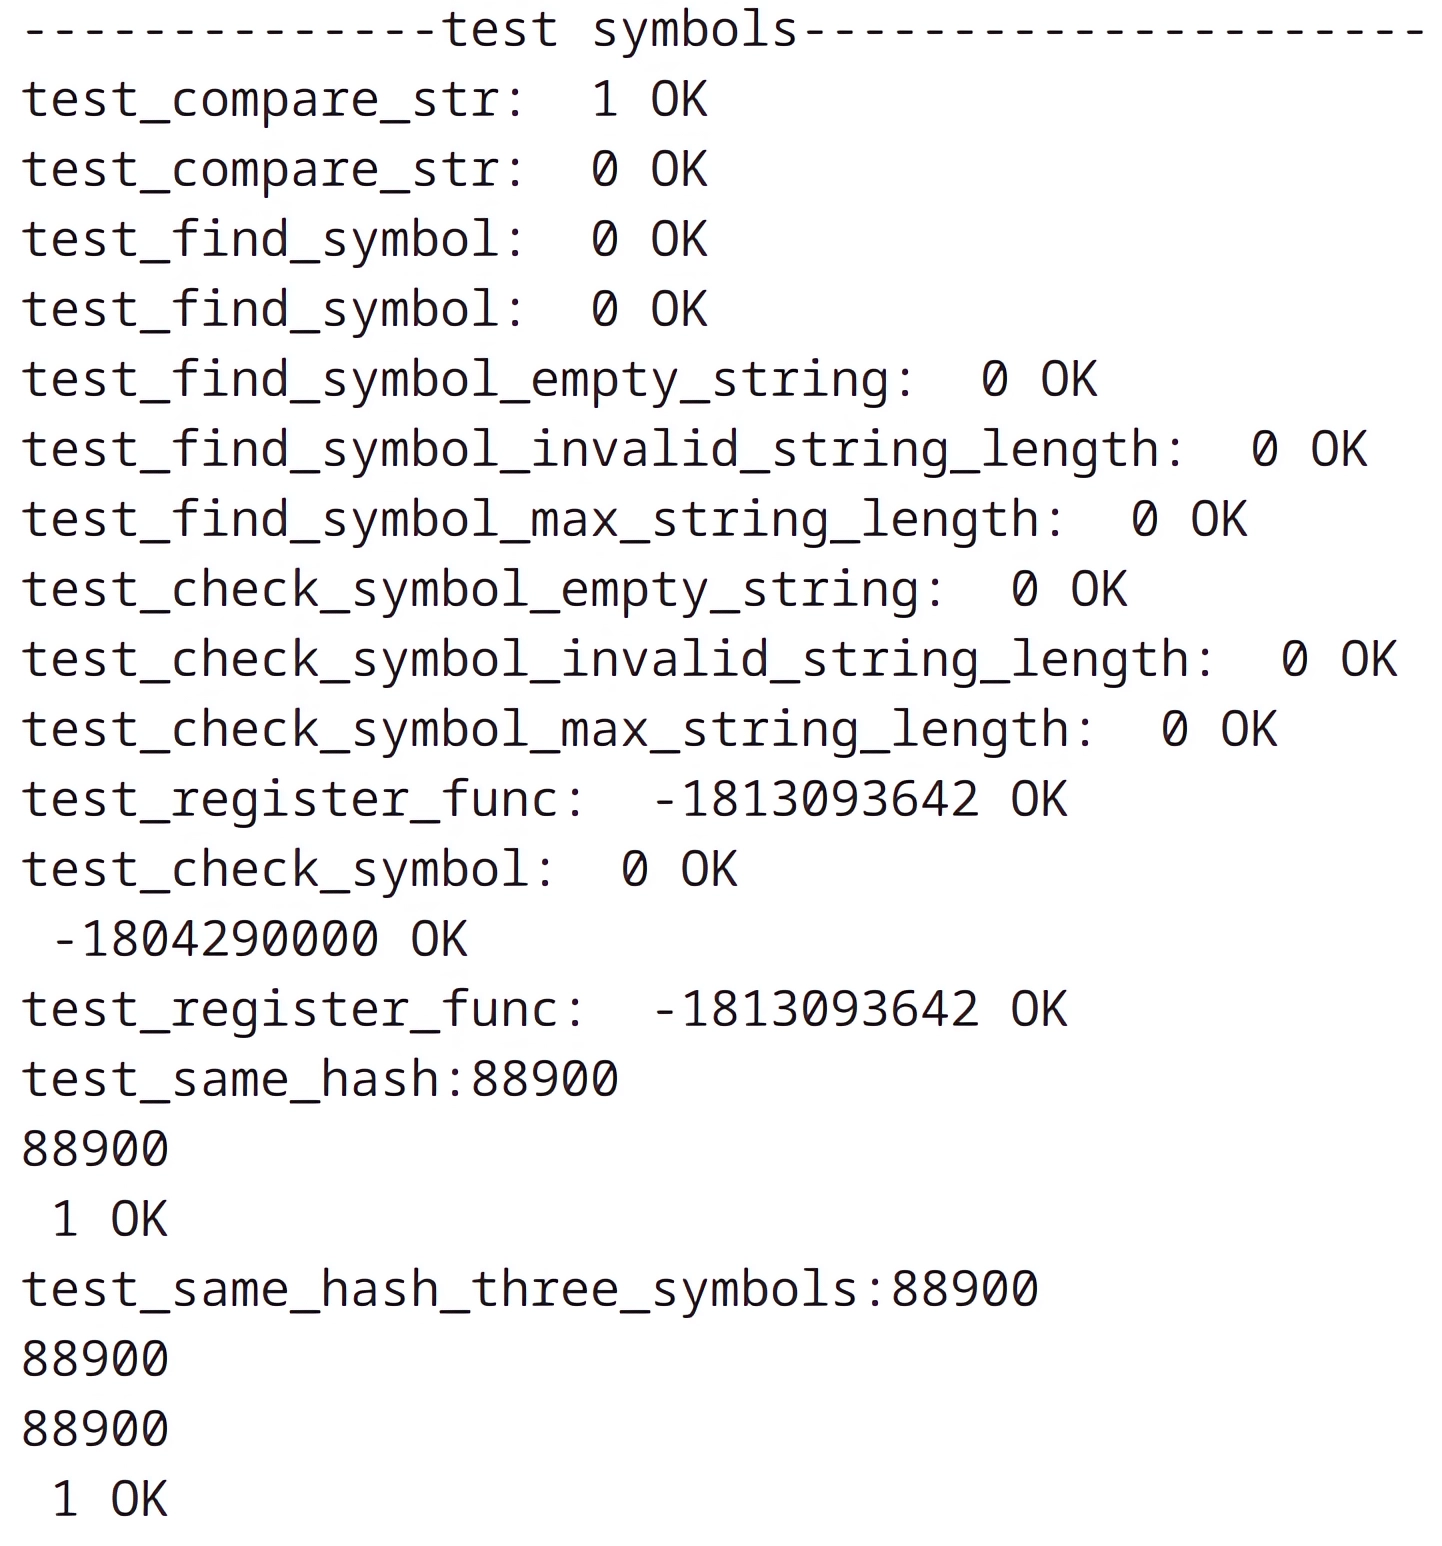
\includegraphics[width=1\linewidth]{modul_test_res}}
	\caption{Вывод в консоль результатов выполнения модульного теста test\_symbols.c}
	\label{modul_test_res:image}
\end{figure}

\subsection{Системное тестирование разработанного интерпретатора}

Системные же тесты проверяют работу ПС по принципу чёрного ящика, с теми же возможностями, что есть у пользователя. Этот метод подходит для проверки корректности работы интерпретатора в целом \cite{e15}. Суть подхода заключается в запуске передаваемого в виде строки программного кода и сравнения выведенных в консоль результатов его выполнения с эталонными.

Для тестирования используется bash-скрипт \quotes{sys\_test}. При его вызове программный код подаётся в двойных кавычках первым аргументом, а эталонный (ожидаемый) результат аналогичным образом вторым аргументом. При совпадении фактического и ожидаемого результата, в поток вывода \cite{e28} попадёт \quotes{OK}, иначе \quotes{FAIL}. Запуск тестового пакета необходимо производить в консольном интерфейсе, запись результатов при этом будет происходить в стандартный поток вывода консоли.

Несколько тестов из пакета системного тестирования представлены на рисунке \ref{system_test_code:image}.

\begin{figure}[ht]
	\center{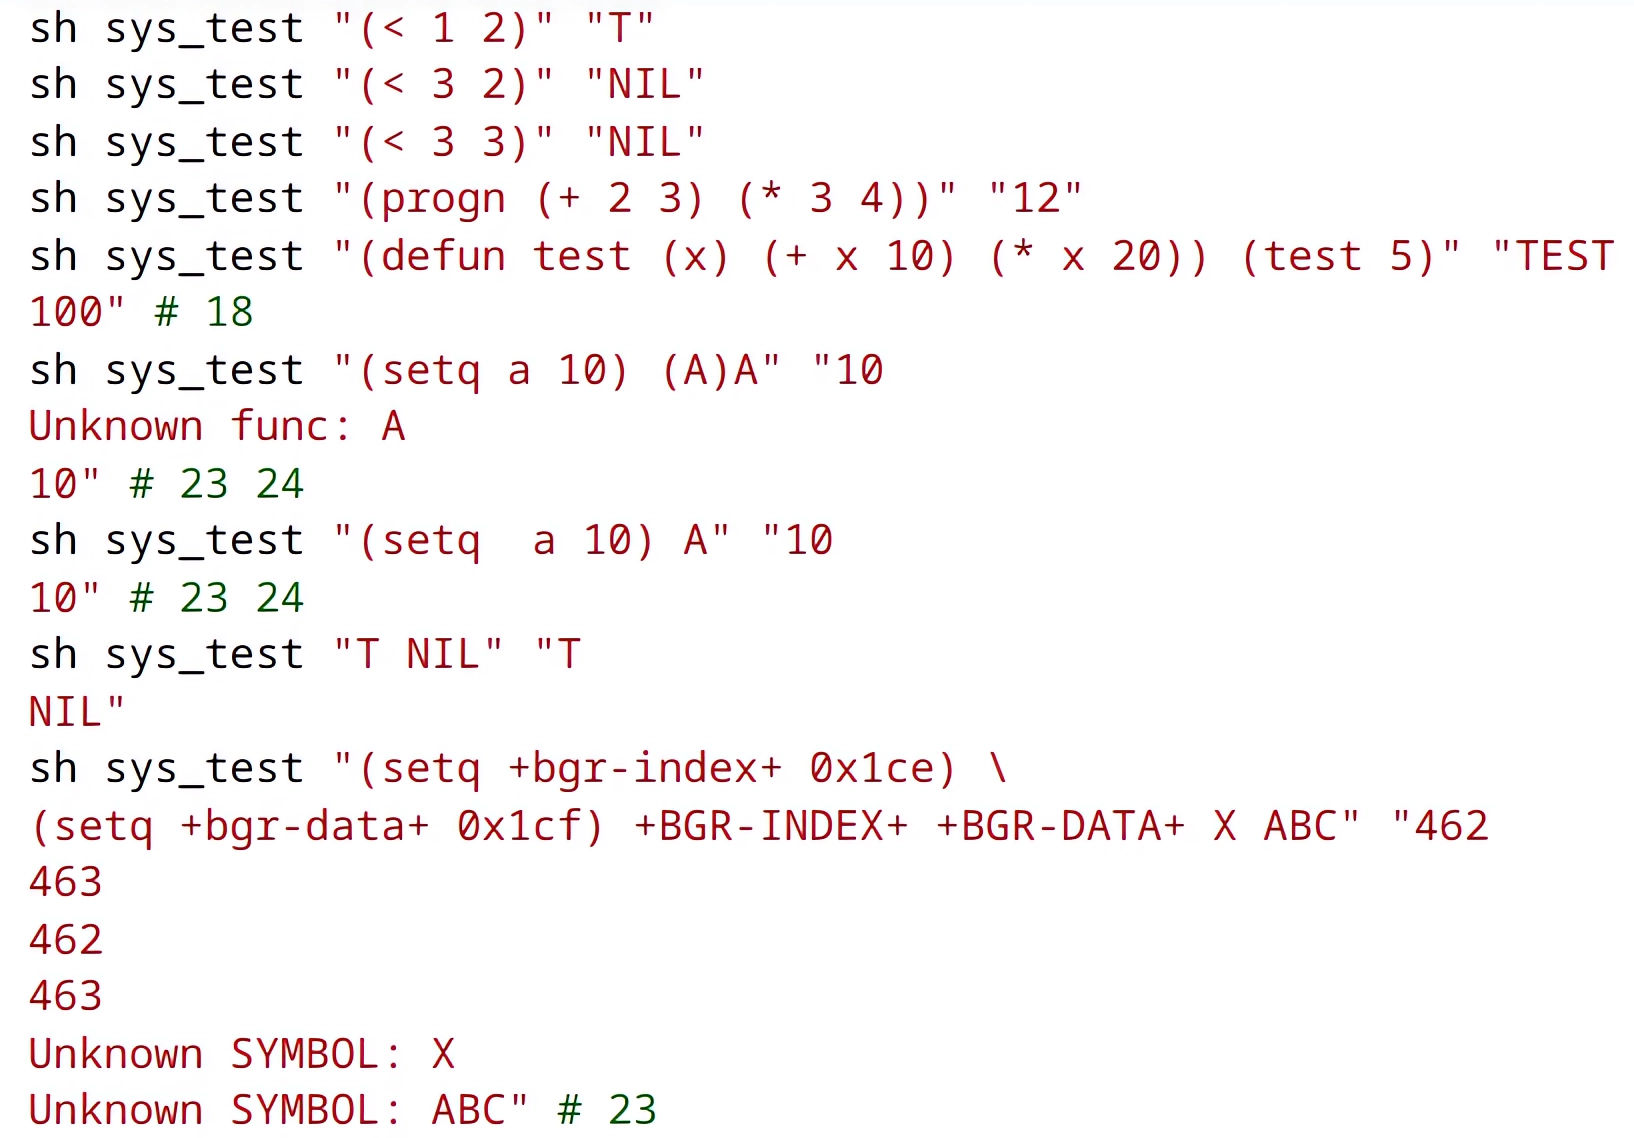
\includegraphics[width=1\linewidth]{system_test_code}}
	\caption{Часть тестов из пакета системного тестирования}
	\label{system_test_code:image}
\end{figure}

Вывод в консоль результатов выполнения этих тестов так же показан на рисунке \ref{system_test_res:image}.

\begin{figure}[ht]
	\center{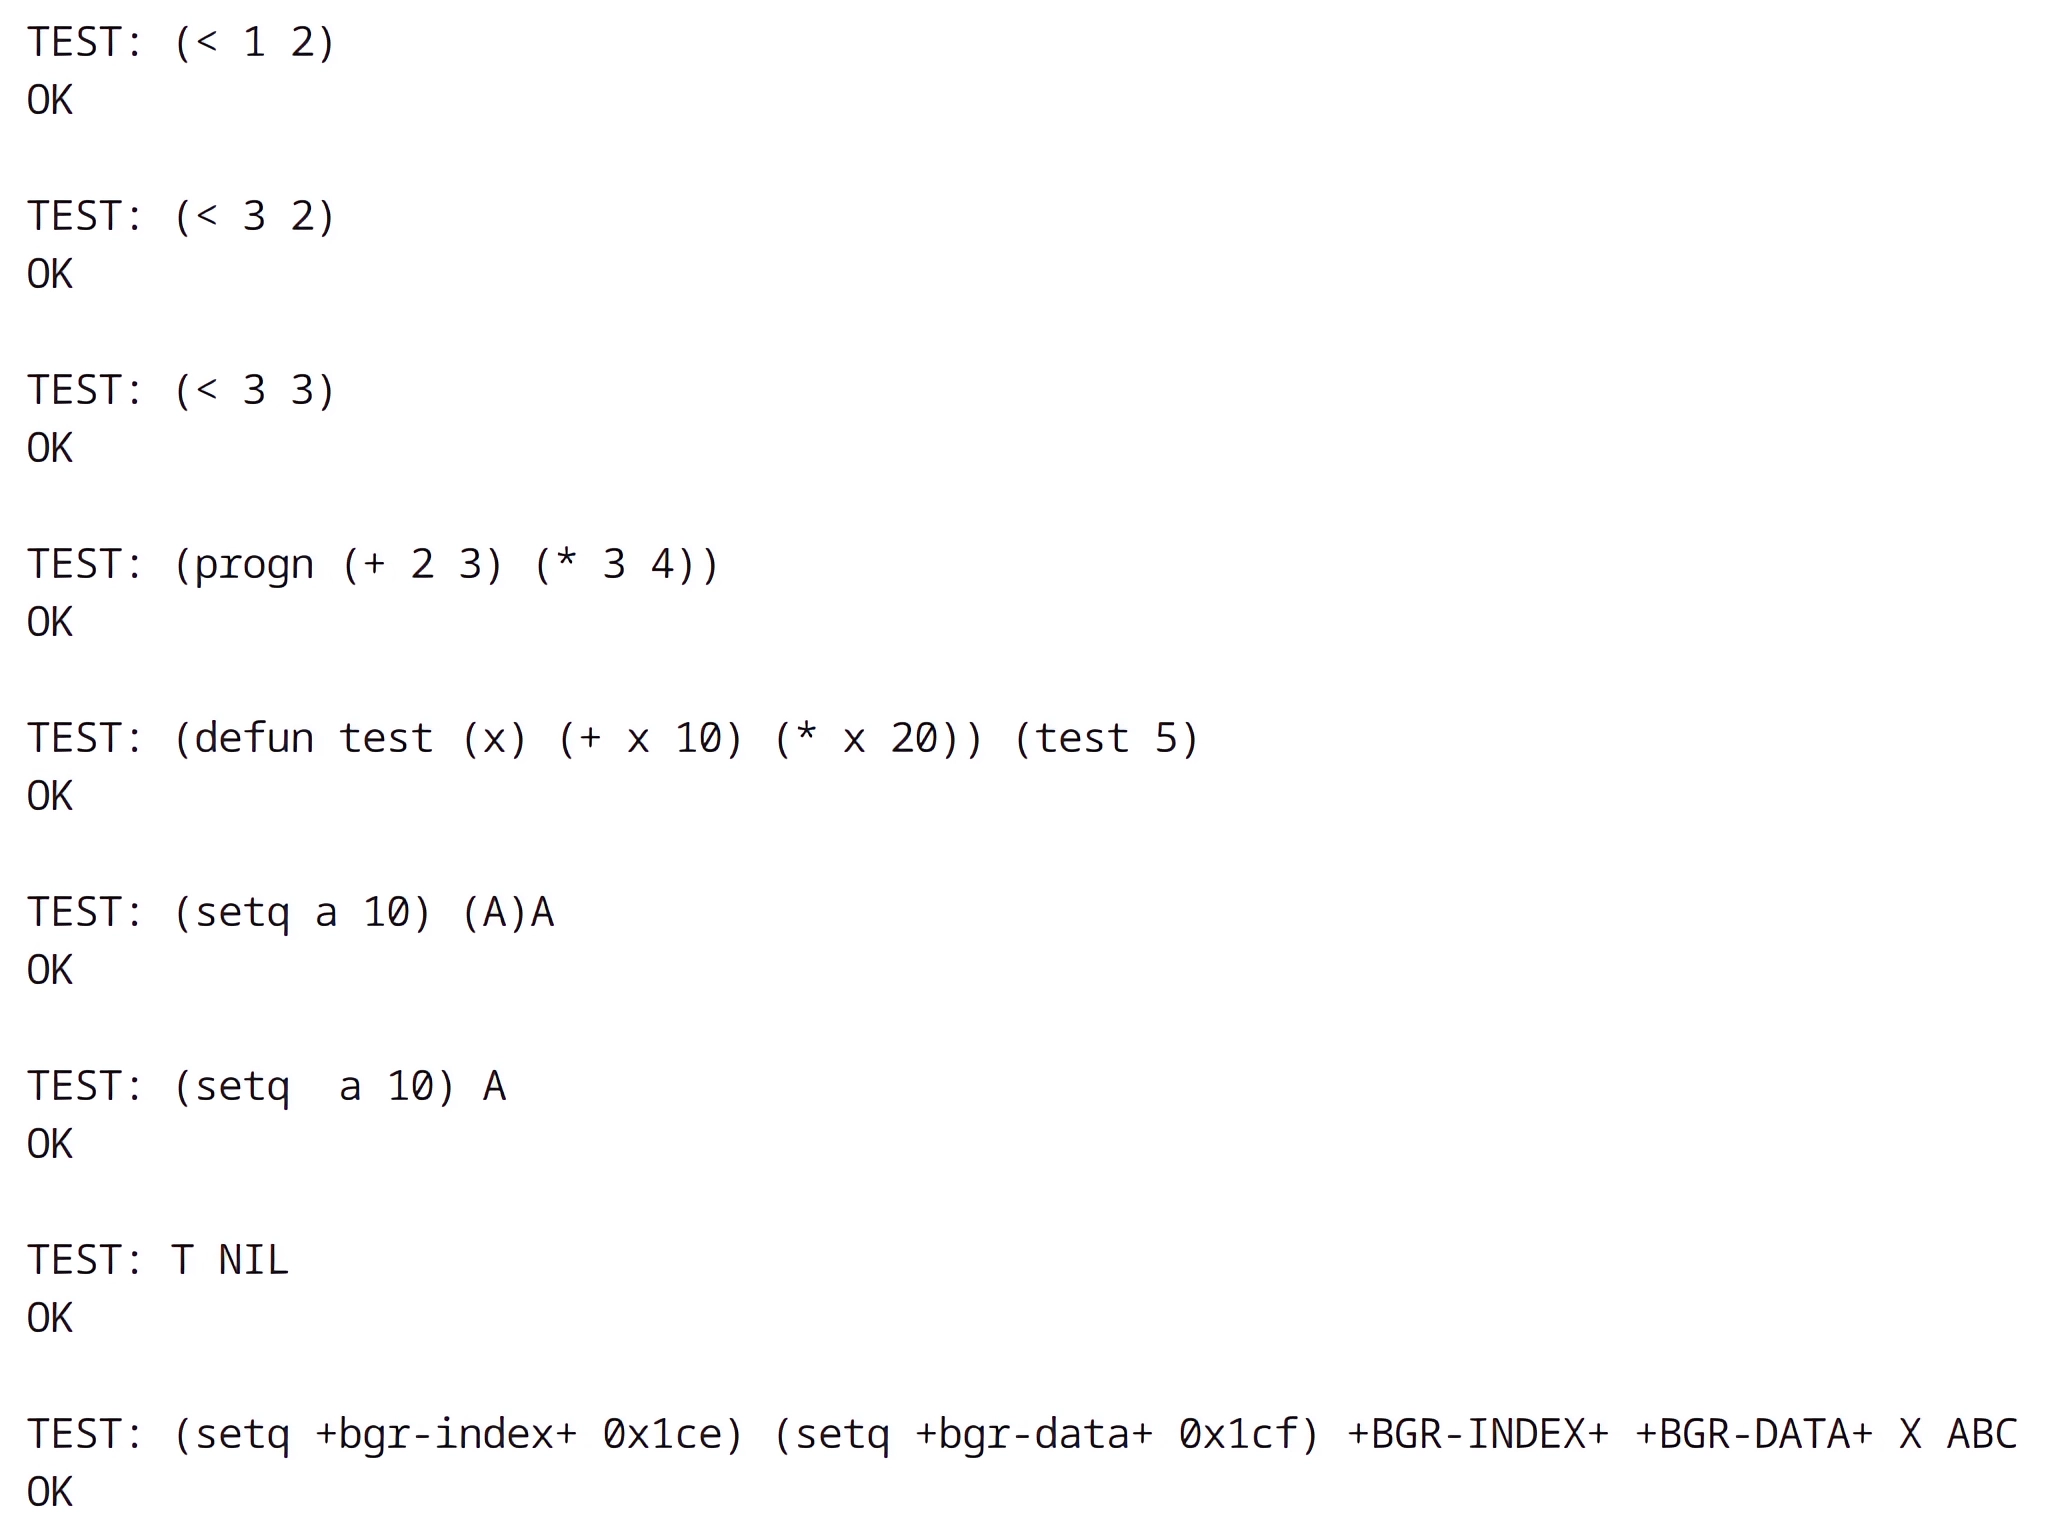
\includegraphics[width=1\linewidth]{system_test_res}}
	\caption{Вывод в консоль результатов выполнения системных тестов}
	\label{system_test_res:image}
\end{figure}

Алгоритм работы тестового пакета:

\begin{enumerate}
\item Определяем переменные \quotes{IN}, \quotes{OUT}, и \quotes{OUT\_EXP}, используемые для хранения путей к временным файлам для хранения кода, фактических результатов и ожидаемых результатов соответственно. В дальнейшем "IN" будет использоваться для передачи программного кода на выполнение, а \quotes{OUT}" и \quotes{OUT\_EXP} для сравнения результатов;

\item Выводим строку \quotes{TEST: \$1}, где \quotes{\$1} — выполняемый программный код;

\item Записываем строку выполняемого программного кода в файл, путь к которому задан в переменной \quotes{IN}. Аналогично поступаем с ожидаемым результатом, но берём путь из переменной \quotes{OUT\_EXP};

\item Запускаем интерпретатор, перенаправляя в его поток вввода данные из файла \quotes{IN}, а также перенаправляем поток вывода в \quotes{OUT};

\item Сравниваем данные из файлов \quotes{OUT} и \quotes{OUT\_EXP}, используя встроенную в систему утилиту \quotes{diff} \cite{e24}. Если файлы идентичны, выводим \quotes{OK} -- успешное завершение теста, иначе \quotes{FAIL} -- несоответствие ожидаемого вывода фактическому.

\item Выводим пустую строку, создав тем самым перенос строки для визуального разделения результатов тестов.

\end{enumerate}

\subsection{Сборка программной системы}
Для компиляции созданной ПС были разработаны два файла сборки \quotes{makefile} \cite{e8}, реализующие разные варианты сборки интерпретатора.

Первый, расположенный в корневой папке разработанного интерпретатора, компилирует все модули интерпретатора в один готовый к использованию исполняемый файл. Для запуска сборки используется команда \quotes{make build}. В результате в той же папке будет сформирован файл \quotes{cl-inter}. Теперь можно запустить интерпретатор с нужным файлом исходного кода программы, передав путь до него в качестве параметра. Например: \quotes{cl-inter ./script}.

Второй, \quotes{test}, предназначен для запуска модульных и системных тестов, при этом, в случае модульного тестирования, в скомпилированный файл входят только необходимые для тестируемого модуля компоненты. Расположен в папке test, где также находятся все файлы тестов. При вызове \quotes{make test} поочерёдно будут собираться и выполняться все разработанные модульные и системный тесты. Исполняемые файлы при этом будут помещены в директорию ОС для временных файлов - \quotes{/tmp} \cite{e25}.
   \section*{ЗАКЛЮЧЕНИЕ}
\addcontentsline{toc}{section}{ЗАКЛЮЧЕНИЕ}

В процессе выполнения данной работы была создана программная система, позволяющая сокращение размера исходного кода программ за счёт метапрограммирования.

Программная система предлагает к использованию возможности функциональной парадигмы и метапрограммирования для повышения скорости разработки, уменьшения объема кода, упрощения масштабирования и обеспечения большей мобильности разрабатываемого ПО.

Основные результаты работы:
\begin{enumerate}
	\item Проведён анализ предметной области;
	\item Спроектирован функциональный язык программирования с поддержкой метапрограммирования, являющийся подмножеством языка \quotes{Common Lisp};
	\item Спроектирован интерпретатор этого языка;
	\item Выбраны технологии и методики для реализации интерпретатора;
	\item Интерпретатор реализован средствами языка программирования \quotes{C} и ОС \quotes{GNU/Linux}.
\end{enumerate}


Все требования, объявленные в техническом задании, были полностью реализованы, все задачи, поставленные в начале разработки проекта, были также решены.

Разработанная программная система была успешно использована для сокращения исходного кода существующей программы путём её переписывания на разработанный язык с применением возможностей метапрограммирования.
}\fi
\addcontentsline{toc}{section}{СПИСОК ИСПОЛЬЗОВАННЫХ ИСТОЧНИКОВ}

\begin{thebibliography}{9}
	
	\bibitem{javascript} Пратт Т., Зелковиц М. Языки программирования: разработка и реализация / Под общей ред. А. Матросова. – СПб.: Питер, 2002. – 688 с.: ил. – ISBN 5–318–00189–0. – Текст~: непосредственный.
	\bibitem{php} Клинтон Л. Джеффери. Создайте свой собственный язык программирования. Руководство программиста по разработке компиляторов, интерпретаторов и доменно–ориентированных языков для решения современных вычислительных задач / пер. с англ. С. В. Минца. – М.: ДМК Пресс, 2023. – 408 с.: ил. – ISBN 978–5–93700–140–5. – Текст~: непосредственный.
	\bibitem{css} Ахо, Альфред В., Лам, Моника С., Сети, Рави, Ульман, Джеффри Д. Компиляторы: принципы, технологии и инструментарий, 2 е изд . : Пер . с англ. – М. : ООО “И.Д. Вильямс”, 2018 – 1184 с. : ил. – ISBN 978–5–8459–1932–8 – Текст~: непосредственный.
	\bibitem{mysql}	Свердлов С. З. Конструирование компиляторов. Учебное пособие // LAP Lambert Academic Publishing, 2015 – 571 стр., ил. – ISBN 978–3–659–71665–2. – Текст~: непосредственный.
	\bibitem{html5}	Хэзфилд Ричард, Кирби Лоуренс и др. Искусство программирования на С. Фундаментальные алгоритмы, структуры данных и примерыприложений. Энциклопедия программиста: Пер. с англ./Ричард Хэзфилд, Лоуренс Кирби и др. –К.: Издательство «ДиаСофт», 2001. – 736 с. – ISBN 966–7393–82–8. – Текст~: непосредственный.
	\bibitem{htmlcss} Костельцев А. В. Построение интерпретаторов и компиляторов : Использование программ BIZON, BYACC, ZUBR : [Учеб. пособие] / А. В. Костельцев. – СПб. : Наука и техника, 2001. – 218,[1] с. : ил. – ISBN 5–94387–033–4. – Текст~: непосредственный.
	\bibitem{bigbook} Шостак, Е. В. Основы программирования трансляторов языков программирования : учеб. – метод. пособие / Е. В. Шостак, И. М. Марина, Д. Е. Оношко. – Минск : БГУИР, 2019. – 66 с. : ил. – ISBN 978–985–543–470–3. – Текст~: непосредственный.
	\bibitem{uchiru} Коробова, И.Л. Основы разработки трансляторов в САПР : учебное пособие / И.Л. Коробова, И.А. Дьяков, Ю.В. Литовка. – Тамбов : Изд–во Тамб. гос. техн. ун–та, 2007 – 80 с. – ISBN 978–5–8265–0591–5. – Текст~: непосредственный.
	\bibitem{chaynik} Ричард Бёрд. Жемчужины проектирования алгоритмов: функциональный подход / Пер. с англ. В. Н. Брагилевского и А. М . Пеленицына. – М .; Д М К Пресс, 2013. – 330 с.: ил. – ISBN 978–5–94074–867–0. – Текст~: непосредственный.    
	\bibitem{22} Сайбель П. Практическое использование Common Lisp / пер. с англ. А.Я. Отта. – М.:ДМК Пресс, 2015. – 488 с.: ил. – ISBN 978–5–94074–627–0. – Текст~: непосредственный.    
	\bibitem{1231}	Форд Н. Продуктивный программист. Как сделать сложное простым, а невозможное – возможным. – Пер. с англ. – СПб.: Символ–Плюс, 2009. – 256 с., ил. – ISBN 978–5–93286–156–1. – Текст~: непосредственный.    
	\bibitem{sdf} Структура и интерпретация компьютерных программ [Текст] / Харольд Абельсон, Джеральд Джей Сассман, при участии Джули Сассман ; [пер. Г. К. Бронникова]. – 2–е изд. – Москва : Добросвет : КДУ, 2012. – 608 с. : ил. – ISBN 978–5–98227–829–6. – Текст~: непосредственный.    
	\bibitem{servsssds}	Лав Р. Linux. Системное программирование. 2–е изд. – СПб.: Питер, 2014. – 448 с.: ил. – ISBN 978–5–496–00747–4. – Текст~: непосредственный.
\end{thebibliography}

\ifВКР{\appendix{Представление графического материала}

Графический материал, выполненный на отдельных листах,
изображен на рисунках А.1--А.\arabic{числоПлакатов}.
\setcounter{числоПлакатов}{0}

\renewcommand{\thefigure}{А.\arabic{figure}} % шаблон номера для плакатов

\begin{landscape}

\begin{плакат}
    \includegraphics[width=0.82\linewidth]{pl1.eps}
    \заголовок{Сведения о ВКРБ}
    \label{pl1:image}      
\end{плакат}

\begin{плакат}
    \includegraphics[width=0.82\linewidth]{pl2.eps}
    \заголовок{Цель и задачи разработки}
    \label{pl2:image}      
\end{плакат}

\begin{плакат}
    \includegraphics[width=0.82\linewidth]{pl3.eps}
    \заголовок{Концептуальная модель функционального языка}
    \label{pl3:image}      
\end{плакат}

\begin{плакат}
    \includegraphics[width=0.82\linewidth]{pl4.eps}
    \заголовок{Архитектура интерпретатора}
    \label{pl4:image}      
\end{плакат}

\begin{плакат}
	\includegraphics[width=0.82\linewidth]{pl5.eps}
	\заголовок{Лексический анализ}
	\label{pl5:image}      
\end{плакат}

\begin{плакат}
	\includegraphics[width=0.82\linewidth]{pl6.eps}
	\заголовок{Синтаксический анализ}
	\label{pl6:image}      
\end{плакат}

\begin{плакат}
	\includegraphics[width=0.82\linewidth]{pl7.eps}
	\заголовок{Вычислитель}
	\label{pl7:image}      
\end{плакат}

\begin{плакат}
	\includegraphics[width=0.82\linewidth]{pl8.eps}
	\заголовок{Примеры макросов операторов}
	\label{pl8:image}      
\end{плакат}

\begin{плакат}
	\includegraphics[width=0.82\linewidth]{pl9.eps}
	\заголовок{Заключение}
	\label{pl9:image}      
\end{плакат}

\end{landscape}
}\fi
\ifПрактика{}\else{\appendix{Фрагменты исходного кода программы}

main.tex
\lstinputlisting[language=Tex, frame=none]{main.tex}

ТехПроект.tex
\lstinputlisting[language=Tex, frame=none]{ТехПроект.tex}

\ifВКР{
\newpage
\addcontentsline{toc}{section}{На отдельных листах (CD-RW в прикрепленном конверте)}
\begin{center}
\textbf{Место для диска}
\end{center}
}\fi
}\fi
\end{document}
